\documentclass[twocolumn]{article}
\usepackage[utf8]{inputenc}
\usepackage{ctex}
\usepackage{stfloats}
\usepackage[T1]{fontenc}
\usepackage[english]{babel}
\usepackage{diagbox}
\usepackage{ifpdf,amsmath,amsthm,amssymb,amsfonts,newtxtext,newtxmath} 
\usepackage{array,graphicx,dcolumn,multirow,hevea,abstract,hanging}
\usepackage[labelfont=sc,textfont=sf]{caption}
\usepackage[hyperfootnotes=false,breaklinks=true]{hyperref} % was dvipdfmx
\urlstyle{rm}
%\usepackage[hyphenbreaks]{breakurl}
\usepackage{apacite} % must come afer hyperfootnotes
\setlength{\bibleftmargin}{1em}
\setlength{\bibindent}{-1em}
\usepackage{booktabs} % \toprule \midrule \bottomrule \cmidrule(lr){a-b}

%%%% Added by Zhenbo Cheng
\usepackage{subcaption}
%%%%%%%%%%%%%%%%%%%%%%%%

% define centered and ragged columns:
\newcolumntype{L}[1]{>{\raggedright\arraybackslash }p{#1}} % can use m{}
\newcolumntype{C}[1]{>{\centering\arraybackslash }p{#1}}
\newcolumntype{R}[1]{>{\raggedleft\arraybackslash }p{#1}}
\newcolumntype{d}[1]{D{.}{.}{#1}} % d{3.2} for 3 places on l, 2 on r
\newcommand{\mc}{\multicolumn}
\topmargin=-.3in \oddsidemargin=-.1in \evensidemargin=-.1in \textheight=9in \textwidth=6.8in
\setlength\tabcolsep{1mm}
\setlength\columnsep{5mm}
\setlength\abovecaptionskip{.5ex}
\setlength\belowcaptionskip{.5ex}
\setlength\belowbottomsep{.3ex}
\setlength\lightrulewidth{.04em}
\renewcommand\arraystretch{1.2}
\renewcommand{\topfraction}{1}
\renewcommand{\textfraction}{0}
\renewcommand{\floatpagefraction}{.9}
% \renewcommand{\baselinestretch}{1.00} \large\normalsize % for fixing spaces
\widowpenalty=1000
\clubpenalty=1000
\setlength{\parskip}{0ex}
\let\tempone\itemize
\let\temptwo\enditemize
\let\tempthree\enumerate
\let\tempfour\endenumerate
\renewenvironment{itemize}{\tempone\setlength{\itemsep}{0pt}}{\temptwo}
\renewenvironment{enumerate}{\tempthree\setlength{\itemsep}{0pt}}{\tempfour}

%%%%%%%%%%%%%%%%%%%%%%%%%%%%%%%%%%%%%%%%%%%%%%%%%%%%%%%%%%%%%%%%%%%%%
\setcounter{page}{1} % start with first page

\title{题目}

\author{
肖刚
\and 
周华康
\and
陈振波
}

% who is corresponding author?

\date{} % leave empty
\begin{document} % goes here

% fill in short title
\newcommand{\jref}{http://journal.sjdm.org/vol13.2.html}
\newcommand{\jhead}{Judgment and Decision Making, Vol.~13, No.~2}
\newcommand{\jdate}{March 2018}
\pagestyle{myheadings} \markright{\protect\small \href{\jref}{\jhead}, \jdate \hfill Strategies of matcching and maxmizing \qquad}
\begin{htmlonly}
\href{\jref}{\jhead}, \jdate, pp.\
\end{htmlonly}
%\begin{latexonly}
\twocolumn[
\vspace{-.3in}
{\small \href{\jref}{\jhead}, \jdate, pp.\ XX--XX}
%\end{latexonly}

\maketitle

%\begin{latexonly}
\vspace{-3mm}
\begin{onecolabstract}
%\end{latexonly}
近年来,用户对无缝切换高清流需求的增长和基于DASH标准的自适应流的广泛采用,成为
码率自适应算法研究的主要驱动力。现有的大部分码率自适应算法通过硬编码实现,无法有效
应对网络环境的变化。此外也有学者提出使用可以获得更高QoE的Q学习的方法来学习得
到优化的码率自适应算法。但Q学习存在难以编码连续的状态值和在大状态空间下算法
收敛速度慢的问题。为此,本文结合了最近邻算法,提出了一个可以处理连续状态的KNN-Q学习
算法。实验结果表明,在码率自适应情境中,KNN-Q学习相比普通Q学习可以获得更高的QoE和
更快的收敛速度。
\smallskip
\noindent
关键词: 
%\begin{latexonly}
\end{onecolabstract}\bigskip
]
%\end{latexonly}


\section{前言}

目前,视频数据正在成为传统互联网,尤其是移动互联网的主流数据。视频数据相比于其它数据
传输需要更高的比特率,因此带来的移动流量增长更为明显。根据思科全球移动数据流量预测
(2016- 2021)白皮书\cite{RN1}显示,到2021年,移动视频将增长8.7倍,占总移动流
量的78%。用户对视频质量和交互特性有了更多的要求。

每天都有成千上万的视频通过HTTP传输。视频数据通过HTTP传输可以轻易通过防火墙和NAT设备。
各大厂商基于HAS(HTTP Adaptive Streaming)技术,也都研发出了适用于各自设备或者客户
端的自适应流媒体传输技术,如Apple的HLS(HTTP Live Streaming),Microsoft的MSS
(Microsoft Silverlight Smooth Streaming)以及Adobe的HDS(HTTP Dynamic Streaming)。
MPEG组织在2011年制定了DASH(Dynamic Adaptive Streaming over HTTP)标准,旨在
统一在不同设备和服务器制造商之间传送动态码率的视频技术标准\cite{RN2}。相比于HLS和MSS,
DASH标准不仅支持多种编码方式,还支持多种厂家的CDN对接。

DASH标准的设计思想是:服务器将原始视频切分成内容相同而码率不同的视频片段,然后生成一个
包含所有视频片段信息和他们下载地址的索引文件MPD(Media Presentation Description)。
客户端下载并解析MDP文件后,在播放过程中
根据当前的视频质量和网络情况切换合适码率的视频片段下载\cite{RN3}。DASH标准开放了码率自适应算法的
设计,使开发者可以实现自己的码率自适应算法来提供更高的QoE(Quality of Experience)。

现有的码率自适应算法大都基于启发式算法,该算法通常使用硬编码的方式根据网络情况选择合适的
码率,会导致无法有效应对网络环境频繁波动的情况\cite{RN4}。Dana等人提出了采用强化学习中Q-Learning
算法来得到优化过后的码率自适应策略\cite{RN5}。该方法相比于启发式算法可以得到更高的QoE,
但在状态划分过于多时,该方法存在难以学习连续的状态值和学习收敛速度慢的不足。针对该问题
本文结合最近邻算法提出了一种KNN-Q学习算法作为获取获取视频片段的策略。实验结果表明KNN-Q学习算法
可以获得更高的QoE。

本文的组织结构:......

\section{相关工作}

客户端接受流媒体必须能够针对网络情况,客户端状态和用户体验自适应选择码率,才能在不同环境下可靠高
效地接受视频。

有研究\cite{RN7}表明用户对画质的提升不敏感,但是常常能够察觉到画质的下降。应该尽量避免频繁改变画质,
即使不能避免画质变化,也需要控制在较小的幅度内变化。与QoE相关的自适应策略往往需要考虑多个方面如可用
带宽、缓存、画质等,以准确反应用户所感知到的QoE。Mok\cite{RN6}等人提出了结合QoE且基于启发式的
码率自适应算法,QDASH-abw模块位于服务器的代理中用以测量当前带宽下可以支持的最高视频质量,
客户端基于QDASH-qoe算法选择最合适的视频质量等级。他们的的实验结果表明用户更喜欢在最好和最坏的视频质量
之间平缓过度,而不是突然切换。Zink\cite{RN7}等人的NOVA自适应策略提出了"cross-layer"旨在权衡
资源分配和码率自适应,使用之前S个视频片段的质量和时间的方差作为衡量QoE的标准。上述基于启发式的码率
自适应算法,无法方便地建立可预测的数学模型,码率选择策略的灵活度较低,在网络情况复杂的环境中,
码率选择算法的稳定性较差。

引入机器学习方法,客户端可以在无人干预的情况下根据前后环境的变化,学习如何调整所请求的视频分块的比特率。
使用机器学习的方法可以增强客户端码率自适应策略的自适应性和灵活性。Chien\cite{RN9}等人基于随机森林
决策树模型将网络状态特征值(如最新分片的带宽,会话的平均带宽和带宽的波动等)映射到优秀的码率自适应
算法所得到的码率标签,最后使用训练好的分类模型预测视频片段的比特率大小。基于有监督学习的
一个缺点在于需要准备训练数据,虽然Chien的算法可以通过在线学习的方法收集用户的数据,但是
由于环境、用户需求和终端设备的多样性,训练出一个针对所有情景鲁棒性较强的模型还是比较困难的。

将强化学习引入DASH的码率自适应算法中,可以使HAS客户端不断与环境交互,根据当前网络环境的反馈训练自身
的策略,动态学习选择最佳动作。相比于有监督学习,强化学习不需要准备大量训练数据,
只需要在学习时定义合理的动作回报函数。Marinca\cite{RN10}
等人在MAC层上实现了一个HAS自学习系统,该系统使用部分可见的马尔可夫模型建模,基于Q学习设计了
一个在线学习的码率自适应算法。Zhu等人\cite{RN11}提出了一个无限时间的马尔可夫模型,在
训练过程中使用Virutal Experience(VR)策略更新Q表。该方法的实验结果表明VR策略加速了模型收敛
的过程,相比于近似最优的启发式算法在网络状态多变的环境中总体上获得了更高的奖励和显著降低了延迟。
Zhang\cite{RN12}等人将QoE的准则定位成总累计比特率、丢包率和视频饥饿时长,构建了一个
考虑QoE的深度自转移强化学习网络(Self-Transfer learning,STL)。STL算法综合了一系列
伪奖励用以训练虚拟决策中心,然后虚拟决策中心不断将学习到的自适应决策传递给原始决策中心,实验
结果表明STL算法可以提高训练效率和泛化性能。在结合深度学习和强化学习的特性之后,Gadaleta等人\cite{RN14}
利用了前馈神经网络和递归神经网络的优点设计了一个D-DASH框架。D-Dash框架使用视频片段质量和视频重缓事件
存评价性能在模拟和真实的环境之下获得了相当高的QoE。

在使用强化学习解决码率自适应的情境之中,需要权衡算法收敛速度和状态划分粒度。状态划分过多,可以增强
系统的健壮性,但会导致迭代时收敛速度过慢;状态划分过于离散,对问题情境的刻画
达不到理想状态,这时收敛速度加快。针对码率自适应情境中,状态都是连续的值,本文提出了
一种结合最近邻和Q-learning的算法。从流媒体的视频质量考虑,综合选择与QoE相关的三个方面:
当时视频片段质量、前后帧视频质量变化和缓存区溢出危险性构建回报函数。实现了基于KNN Q-learing的可以
对连续状态进行码率自适应动作的算法。并且设计了一个仿真实验用于比较普通Q学习和本文所提出的
KNN-Q学习的性能表现。

\section{基于KNN-Q的码率自适应算法}

普通基于时序的DASH客户端会在请求下一个视频片段时使用探索策略
来选择合适的码率。本文使用了基于强化学习的智能体来完成这个探索的过程,帮助DASH客户端
来进行决策。

强化学习是机器学习的一种,由于对智能体来说环境部分可见,导致智能体应对环境做决策的
时候的不确定性。但是与环境互动是智能体唯一学习和成长的方法。智能体在每一步动作之后
都会接收到来自环境的奖励,智能体理解了奖励之后进行下一步的决策。智能体的目标是在
给定环境之中选取最优的行动以最大化累积奖励。\cite{RN13}

在码率自适应算法中,定义DASH客户端为智能体,智能体观察到的环境值定义为状态s,DASH客户端
在某一时刻对某一码率的视频片段请求下载记为动作a。当开始探索时,智能体会更新当前环境的状态。
在Q学习中,Q表相当于智能体的大脑来帮助智能体做出决策。Q函数用于评价当前状态下每个动作的
好坏。如等式1所示智能体在状态s选择动作a,并且获得环境所给的奖励r之后如何更新Q值。
其中$\eta\in\left[0;1\right]$为学习率,代表新值取代旧值的程度;$\lambda\in\left[0;1\right]$
为折扣因子,衡量未来奖励的重要程度。在环境状态划分过细的情况下,使用该方法更新Q表,
会带来收敛速度过慢的问题。码率自适应情境下环境状态都是连续值,本文基于KNN算法,将当前环境状态
前后连续的若干个状态按一定策略一起更新,可以达到加快迭代速率和获得更高累积奖励的效果。(参见3.4)
\begin{equation}
\begin{aligned}
 &\left(1-\eta\right)Q_{old}\left(s_t,a_t\right)+\eta\left[r_{t+1}+\lambda max Q\left(s_{t+1},a\right)\right]\\    
 &\Rightarrow Q_{new}\left(s_t,a_t\right)
\end{aligned}
\end{equation}

每次迭代训练智能体根据之前学习到的Q值,选择合适码率视频片段下载,具体的选择策略参见3.3。环境当前
动作所给的奖励根据
奖励函数计算(参见3.2)。在多次迭代训练之后,会生成一个收敛的Q表。DASH客户端根据当前所处环境选择合
适码率下载视频的时候,查询最终生成的Q表进行决策。下载当前视频片段后会将视频片段加入缓存队列,用以
应对网络异常等特殊情况,最后播放视频队列。

\subsection{环境建模}
DASH客户端需要收集当前可见的环境状态来构建相应的回报函数,并根据相应的策略做出动作。下面将对
环境状态建模和定义DASH客户端的动作行为。
\subsubsection{环境状态}
本文使用三个状态分量来定义环境状态:可用带宽,缓存区总时长和前一个视频片段的视频质量。
可用带宽为DASH客户端测量出来的可用带宽;缓存区总时长代表DASH客户端缓存视频片段的填充状态。这三个状态分量
最终合成的状态定义为$s_t=(BW_t,B_t,q_t-1)$。具体的状态分量的取值范围和离散级别如表\ref{environment state}所示。
\begin{table}[h]
\centering
\renewcommand\arraystretch{0.8}
\caption{环境状态定义}
\label{environment state}
\begin{tabular}{ccc}
\toprule
状态元素& 范围& 级别\\
\midrule
Bandwidth& $\left[0;BW_{max}\right]bps$& $N+1$\\
Buffer filling& $\left[0;B_{max}\right]sec$& $\frac{B_{max}}{T_{seg}}$\\
Quality Level(SSIM)&$\left[-1;1\right]$&$N$\\
\bottomrule
\end{tabular}
\end{table}

如表1所示,$BW_{max}$代表最高可用带宽,$B_{max}$表示缓存区最多可以储存的视频时长,$N$表示码率等级总个数。
前一个视频片段质量的计算方法采用SSIM评价(计算方式参见3.2.1小节)。
\subsubsection{动作}
将DASH客户端的动作定义为对某一码率的视频片段请求下载。可供DASH客户端选择视频片段的下载码率,
由DASH客户端的转码模块事先确定。
\subsection{回报函数}
在强化学习中,回报函数是智能体学习策略经验的基本指南。在流媒体自适应情境中,回报函数一般用来衡量QoE,
但是评价QoE的高低往往带有主观性。比如,无法比较一个在高低质量之间波动的视频和一个稳定在中等质量视频
的好坏。所以使用数学模型来准确衡量QoE很有必要。本文从当前视频片段质量,视频片段质量波动和缓存区溢出
危险性三个方面来构建回报函数。
\subsubsection{视频质量}
本文使用广泛应用于评价视频质量的SSIM作为评价视频质量的指标\cite{RN15,RN16,RN17}。SSIM是衡量两张图片相似度的指标,利用结构
信息来评估图像质量。SSIM的具体计算方式如等式2所示,对于给定的图像$X$和$Y$,利用两个图像中的像素点
亮度的均值、方差和协方差来计算SSIM值。其中$\mu_{X}$和$\mu_{Y}$分别是图像$X$和$Y$的像素点
亮度均值,$\sigma_{X}^2$和$\sigma_{Y}^2$分别是图像$X$和$Y$的像素点亮度值的方差,$\sigma_{XY}$是
图像$X$和$Y$的像素点亮度值之间的协方差,$c_{1}$和$c_{2}$是为了避免分母为零而设置的常数。SSIM$\in\left[-1,1\right]$
,当SSIM越接近1时表示两个图像相似度越高。
\begin{equation}
SSIM\left(X,Y\right)=\frac{\left(2\mu_{X}\mu_{Y}+c_{1}\right)\left(2\sigma_{XY}+c_{2}\right)}
{\left(\mu_{X}^2+\mu_{Y}^2+c_{1}\right)\left(\sigma_{X}^2+\sigma_{Y}^2+c_{2}\right)}
\end{equation}

利用等式2,计算待下载码率的视频片段和原视频片段各帧的SSIM均值用来衡量该视频片段的质量。如等式3所示,用
视频片段的平均SSIM来表示视频片段的质量,其中$m$表示视频片段由$m$帧图片构成,$q_{n}$表示第n个片段的视频质量。
\begin{equation}
q_{n}=\frac{\sum_{i=0}^m SSIM(download_{seg(i)},origin_{seg(i)})}{m}
\end{equation}

如等式4所示,用第n个片段的视频质量来表示DASH客户端下载该视频质量的视频片段所带来的回报值。
\begin{equation}
R_{quality}=q_{n}
\end{equation}
\subsubsection{视频质量振荡}
在网络带宽变化时,DASH客户端请求的视频质量也会发生变化,而视频质量的振荡会带来QoE的下降。
如等式5所示,视频播放期间
质量切换带来的回报损失记为$R_{quality-change}$,根据振荡的步长$\alpha$映射成惩罚回报。
\begin{equation}
R_{quality-change}=-\alpha\left|q_{n}-q_{n-1}\right|
\end{equation}
\subsubsection{缓存区安全性}
本文设置该惩罚项目的在于度量缓存区安全性,如等式6、7和8所示,该惩罚项由安全缓存水平惩罚项和低缓存惩罚项组成。
其中$B_{max}$表示缓存区最大缓存容量,$B_{n}$表示在下载第n个视频片段时缓存区拥有的视频片段的时长,
$\beta$和$\gamma$代表了对缓存安全和缓存安全的关注程度。
在下一个下载动作会引起视频冻结时,$R_{buffer-safe}$的值会明显下降,即惩罚会引起缓存饥饿的行为。DASH客户端
缓存区时长越少的时候,$R_{buffer-low}$的值越小,即惩罚低缓存的行为。
\begin{equation}
R_{buffer-filling}=R_{buffer-safe}+R_{buffer-low}
\end{equation}
\begin{equation}
R_{buffer-safe}=-min\left\{\beta\left(max\left[0,T_{download}-B_{n}\right]\right),1\right\}
\end{equation}
\begin{equation}
R_{buffer-low}=-\gamma\left(max\left[B_{max}-B_{n+1},0\right]\right)^2
\end{equation}
\subsubsection{总回报函数}
总回报函数会推动DASH客户端探索较高的码率等级、较少的码率切换和较合理的缓存数据量的行为决策。
由于QoE往往带有主观性,设置可调的参数很有必要。
如等式9所示,本文设置了$C_{1}$、$C_{2}$和$C_{3}$分别对应$R_{quality}$、
$R_{quality-change}$和$R_{buffer-filling}$的权重,根据所侧重的QoE方面来设置具体的值。
\begin{equation}
R=C_{1}R_{quality}+C_{2}R_{quality-change}+C_{3}R_{buffer-filling}
\end{equation}
\subsection{探索策略}
强化学习的过程中的动作选择需要注意探索和利用的平衡。智能体为了获得更高的累积最大奖励,往往
会选择之前执行过的即时奖励比较大动作;另一方面,智能体需要尝试之前没有被执行过有可能返回
更大即时奖励的动作。专注于探索可能会对短期收益产生影响,专注于利用可以使长期收益最大化,
但往往可能得到的不是最优解。常用的解决方法有$\varepsilon$-greedy方法和Softmax方法\cite{RN18}。

本文采用$\varepsilon$-greedy算法进行探索和利用的平衡。探索过程中以$\varepsilon(0\leq\varepsilon\leq1)$
的概率随机选择下一步的行为,以$1-\varepsilon$的概率选择会带来最大长期回报的行为。
\subsection{KNN-Q算法实现}
\subsubsection{状态划分}
在传统Q学习中,需要将连续的状态类型依据其可取范围划分成若干个状态。设网络状态为$BD_{t}$、
缓存$B_{t}$、前一个视频片段质量$q_{t-1}$各自划分成M、N、L个状态,如图\ref{q-learning state}所示。但传统的Q
学习存在状态划分问题:如果状态划分足够细,可以更精确地描述问题,但算法收敛速度过慢;如果
状态划分粒度太大,虽然能够加快迭代速度,但使对环境建模不准确导致算法表现较差。如何准确的
划分状态成为一个难点。

如图\ref{knn-q-learning state}所示,本文所提出的KNN-Q学习与传统状态划分不同的是,当取值正好为每个区间的中间值时才认定
找到状态,否者该状态的Q值根据邻近状态的Q值计算得到。总状态之间的距离$d_{i}$是根据各个状态
分量的欧式距离计算得出来的,如公式10所示。

\begin{figure*}[ht]
\centering
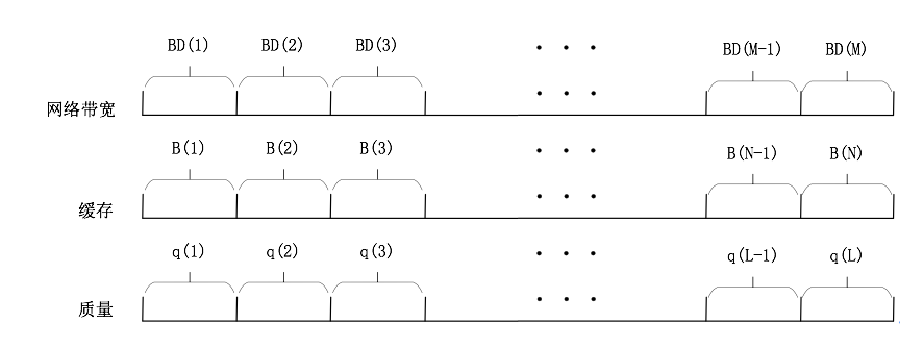
\includegraphics[width=0.8\textwidth]{q-state}
\caption{Q学习状态划分}
\label{q-learning state}
\end{figure*}
\begin{figure*}[ht]
\centering
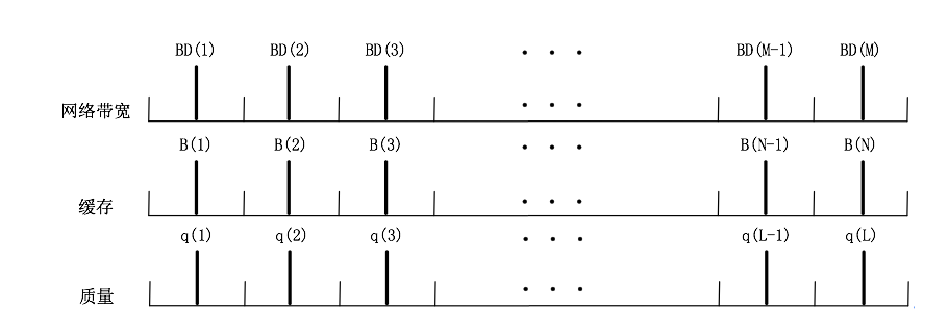
\includegraphics[width=0.8\textwidth]{knn-q-state}
\caption{KNN-Q学习状态划分}
\label{knn-q-learning state}
\end{figure*}
\begin{equation}
d_{i}=\sqrt{(d_{i}^{bandwidth})^2+(d_{i}^{buffer})^2+(d_{i}^{previous-ssim})^2}
\end{equation}

状态$s_{t}$与各个表中状态的邻近状态距离得到之后,从中选出K个距离最小的状态,用
他们的Q值数组计算$s_{t}$的Q值数组,如公式11所示。
\begin{equation}
Q(s_{t},:)=\left\{
\begin{array}{lr}
    Q(s_{t},:),s_{t}\in S\\
    \sum_{i=1}^K w_{i}Q(s^{(i)},a),s_{t}\notin S 
\end{array}
\right.
\end{equation}

$s_{t}\in S$代表$s_{t}$存在状态表中,$s_{t}\notin S$代表状态$s_{t}$在状态表查询不到。
$s^{(i)}$是与状态$s_{t}$相邻近的状态。$w_i$代表了邻近状态$s^{(i)}$其Q值的比重。若$s^{(i)}$
离$s_{t}$的距离$d_i$越小,$w_i$越大;反之,若$s^{(i)}$离$s_{t}$的距离越大,$w_i$越小,
具体计算方式见公式12、13。
\begin{equation}
w_{i}=\frac{\rho _{i}}{\sum\rho_{i}}
\end{equation}
\begin{equation}
\rho_{i}=\frac{1}{d_{i}}
\end{equation}
\subsubsection{Q表更新}
动作执行完成之后,需要根据返回的即使奖励和新的状态更新Q表。如果当前状态可以在状态划分表中找到,则使用
公式1更新Q表。若当前状态无法在状态划分表中找到,则更新K个邻接状态在Q表中的Q值。
\begin{equation}
Q(s^{(i)},a)_{t+1}\leftarrow Q(s^{(i)},a)_{t}+\lambda\theta w_{i}
\end{equation}

其中,$\theta$的计算方式见公式15。$s^{(i)^{\prime}},i=1,......,K$是与状态$s_{t}$下一状态
相邻近的K个状态。基于KNN-Q学习的码率自适应算法在训练阶段的伪代码见表\ref{KNN-Q training}
\begin{equation}
\theta=R_{total}^{(s,a)}+\gamma max x_{a^\prime}\sum w_{i}^{\prime}Q(s^{(i)^{\prime}},a^{\prime})-\sum w_{i}Q(s^{(i)},a)
\end{equation}
\begin{table*}[htbp]
\renewcommand\arraystretch{0.8}
\centering
\caption{KNN-Q训练算法流程伪代码}
\label{KNN-Q training}
\begin{tabular}{l}
\toprule 
\textbf{Input}:The current environment information\\
\textbf{Output}:The learned Q table\\
\midrule 
1.\textbf{Initialize}:  \textbf{SET} Q(S,A) arbitrarily;\\
2.\textbf{REPEAT}(for each episode)\\     
3.\hspace{1cm}$s_{t}$ = Observe current state;\\
4.\hspace{1cm}\textbf{REPEAT}(for each step of episode)\\
5.\hspace{2cm}Choose Q value array Q($s_{t}$,:) from Q(S,A) with formula (11)\\
6.\hspace{2cm}Confirm bitrate to download with Q( ,:) using $\varepsilon$-greedy policy\\
7.\hspace{2cm}Request to download the video segment of the bitrate above;\\
8.\hspace{2cm}Update Buffer $buffer_{t}$ ;\\
9.\hspace{2cm}Calculate the Reward $R_{t}$ with formula (9); \\
10.\hspace{2cm}IF $s_{t}\in S$ \\
11.\hspace{3cm}Update Q(S,A) with formula (1);\\
12.\hspace{2cm}ELSE\\
13.\hspace{3cm}Update Q(S,A) with formula (15);\\
14.\hspace{2cm}END\\
15.\hspace{2cm}$s_{t+1}$ = Observe next state;\\
16.\hspace{2cm}$s_{t}$ = $s_{t+1}$;\\
17.\hspace{1cm}\textbf{UNTILE} reach the end of an epiode\\
18.\textbf{UNTILE} run out the episodes\\
\bottomrule 
\end{tabular}
\end{table*}
\section{仿真实验}
本文通过Matlab来进行一系列仿真实验来评估对比本文提出的KNN-Q学习
与传统Q学习算法性能。使用Matlab编写程序来模拟DASH客户端向服务器
请求下载视频并播放的过程。本文设置DASH客户端在不同带宽条件下,
服务器拥有不同码率视频的条件下来模拟不同的实验所需的场景。并对
本文所提出的KNN-Q学习的K值灵敏度做了对比分析。
\subsection{视频评价指标}
逐帧计算SSIM值非常耗时,为方便起见,本文把视频质量的评价指标SSIM值
近似为以视频相对码率对数值为自变量的多项式\cite{RN19}。不同码率的视频片段的SSIM值
可以由等式16、17得到。
\begin{equation}
\rho_{i}=log\left(\frac{R_{i}}{R_{1}}\right)
\end{equation}
\begin{equation}
SSIM_{i}\simeq1+d_{(1,v)}\rho_{i}+d_{(2,v)}\rho^2+d_{(3,v)}\rho^3+d_{(4,v)}\rho^4
\end{equation}

其中,$R_{1}$是视频的原始码率,$R_{i}$是经过服务器压缩的码率。等式17中
向量$\left[1,d_{(1,v)},d_{(2,v)},d_{(3,v)},d_{(4,v)}\right]$
代表了视频的复杂度。
\subsection{测试视频}
仿真实验中,测试实验视频由多个视频场景组成,单个视频场景的视频复杂度是
恒定的,每个场景时长满足随机指数分布。测试视频包括800个视频片段,每个
视频片段的内容时长为2秒。

仿真实验中用以组成测试视频的视频素材源于EvalVid CIF提供的视频数据集\cite{RN20}。
视频素材库中各个视频素材的$\rho_{i}$与SSIM值的关系如图\ref{Video material bit rate-quality curve}所示。

本文从视频素材库中选取了具有代表性的5个视频素材
(在图\ref{Video material bit rate-quality curve}中用较粗的线条标出),
通过随机组合拼接成完整的测试视频。这5个视频素材分别是 Brutta,
News,Bridge(far),Harbour和Husky。通过最大似然估计发得到5个视频素材的复
杂度系数如表\ref{complexity coefficient matrix}所示。
\begin{figure}[htb]
\centering
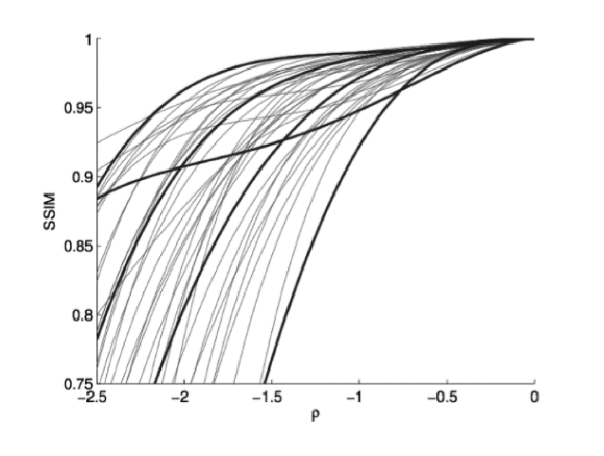
\includegraphics[width=0.8\columnwidth]{complexity}
\caption{视频素材比特率-质量曲线}
\cite{RN19}
\label{Video material bit rate-quality curve}
\end{figure}
\begin{table*}[htbp]
\renewcommand\arraystretch{0.8}
\centering
\caption{5个视频素材的复杂度系数矩阵}
\label{complexity coefficient matrix}
\begin{tabular}{cc}
\toprule 
视频名称&复杂度系数矩阵\\
&$\left[1,d_{(1,v)},d_{(2,v)},d_{(3,v)},d_{(4,v)}\right]$\\
\midrule
Brutta&[-0.0101529,-0.0288832,-0.0242726,0.0041539]\\
News&[-0.0106444,-0.0229079, -0.0253096, 0.0007417]\\
Bridge(far)&[-0.01050829,-0.0538481, -0.0821086, 0.0136133]\\
Harbour&[-0.0050534,0.0055396, -0.01726018, 0.0002203]\\
Husky&[0.0099785,0.0759046,-0.0113807,0.0003986]\\
\bottomrule 
\end{tabular}
\end{table*}
\begin{table*}[htb]
\renewcommand\arraystretch{0.8}
\centering
\caption{5个视频素材各个比特率下的SSIM值}
\label{the SSIM value at each bit rate of 5 video materials}
\begin{tabular}{ccccccccc}
\toprule 
\diagbox{视频}{比特率}&10000&6000&4000&3000&2000&1000&500&300\\
\midrule
Brutta&1&0.99765&0.99554&0.99403&0.99215&0.98977&0.98750&0.98425\\
News&1&0.99851&0.99657&0.99487&0.99209&0.98591&0.97584&0.96352\\
Bridge(far)&1&0.99382&0.98504&0.97767&0.966578&0.94795&0.93211&0.92284\\
Harbour&1&0.99880&0.99647&0.99376&0.98808&0.97169&0.94359&0.91266\\
Husky&1&0.99838&0.99334&0.98641&0.97046&0.92216&0.84148&0.758424\\
\bottomrule 
\end{tabular}
\end{table*}
\subsection{仿真实验参数设置}
\begin{table}[htbp]
\centering
\renewcommand\arraystretch{0.8}
\caption{仿真实验通用参数表}
\label{general parameters}
\begin{tabular}{cc}
\toprule 
参数名&取值\\
\midrule
$\eta$&0.3\\
$\lambda$&0.95\\
$\varepsilon$&0.3\\
K&2\\
$B_{max}$&20sec\\
TrainEpisodes&50\\
TestEpisodes&150\\
StepsOfEpisode&800\\
\bottomrule 
\end{tabular}
\end{table}
仿真实验各场景的参数取值如表\ref{general parameters}所示。
其中$\eta,\lambda$分别是公式1的学习速率和奖励折扣系数。K是
KNN-Q学习中邻接状态的个数,$B_{max}$是DASH客户端的缓存上限。

为避免偶然现象,进行10组重复实验。每组实验包括50个迭代训练
和一次包含150次迭代的测试。每个迭代进行800次步长的训练或测试。
\subsection{实验结果与分析}
DASH客户端在下载视频的过程中,缓存大小会对QoE产生一定影响,同时SSIM值也是衡量视频质量的一个重要指标。
缓存过多时,视频缓存会溢出缓存区;缓存过少时,
在网络情况较差的环境下会引发缓存饥饿,视频画面冻结。
\subsubsection{简单场景}
简单场景模拟了网络带宽比较稳定,但视频内容比较单一的情形。比如当前用户正在播放一望无际的蓝色天空的视频,
此时视频中的场景几乎无变化。故在仿真实验中,该场景下只利用1个视频素材News生成复杂度单一的测试视频。
简单场景中网络带宽变化的范围为$\left[5000,6000\right]$,单位kb/s。

简单场景下DASH客户端的缓存和视频质量对比情况如图\ref{simple_buffer_compare}、
\ref{simple_buffer_bar_graph}所示。在简单场景下,基于KNN-Q学习的码率自适应算法
与传统Q学习的自适应算法缓存增长趋势相同,但是10次实验的平均缓存没有基于Q学习的
自适应算法大。

如图\ref{simple_ssim_compare}、\ref{simple_ssim_bar_graph}所示,
简单场景下,基于KNN-Q学习的码率自适应算法平均的视频质量比传统Q学习的码率自适
应算法高。
\begin{figure}[htbp]
\centering
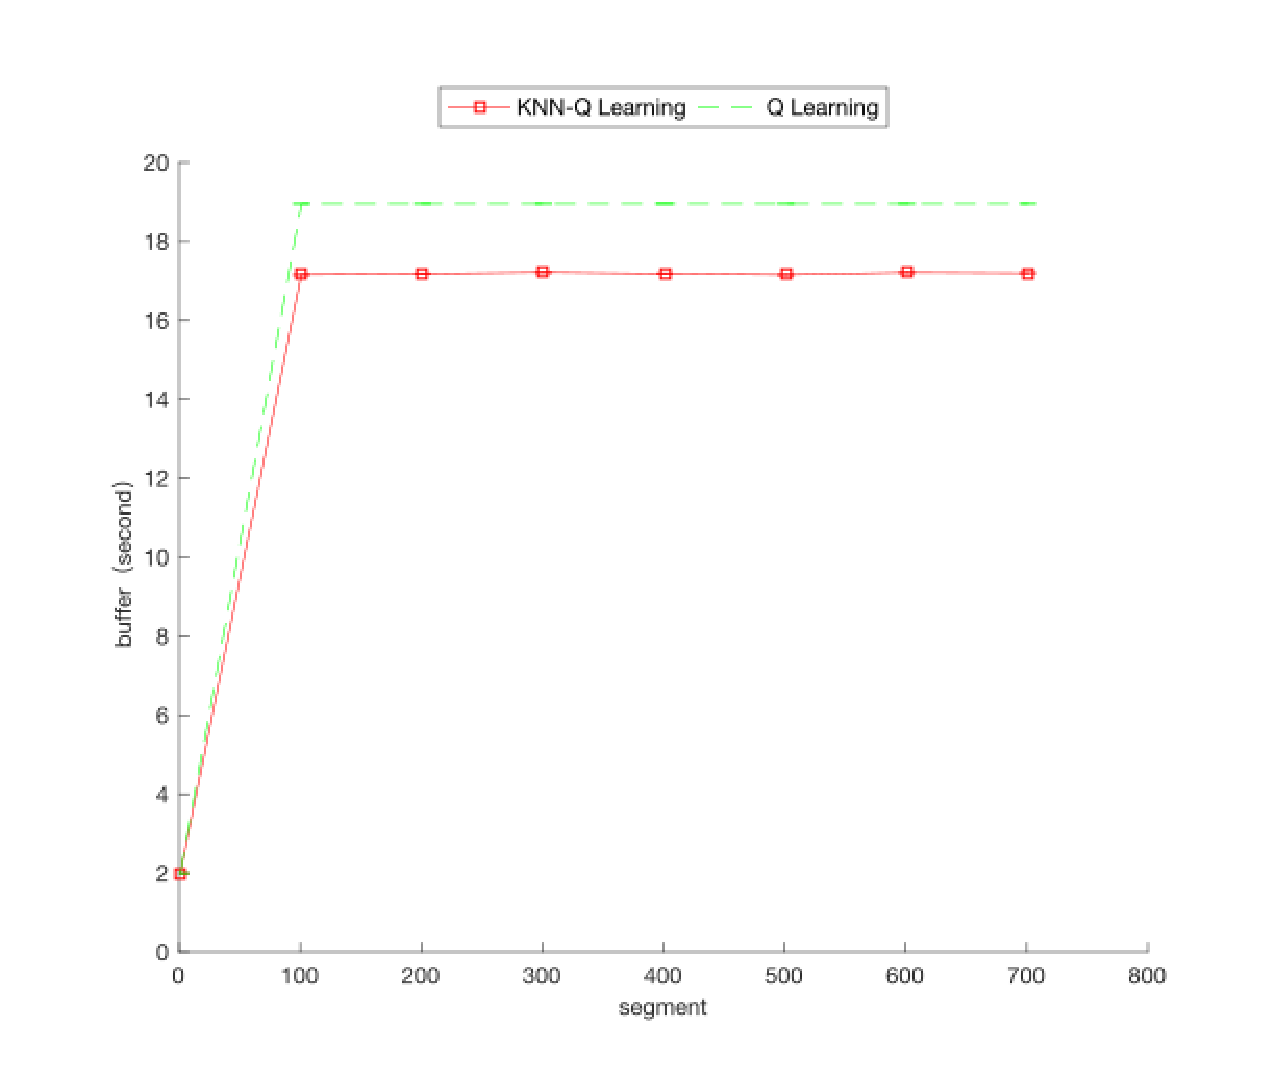
\includegraphics[width=\columnwidth]{simple_buffer_compare}
\caption{简单场景buffer趋势图}
\label{simple_buffer_compare}
\end{figure}
\begin{figure}[htbp]
\centering
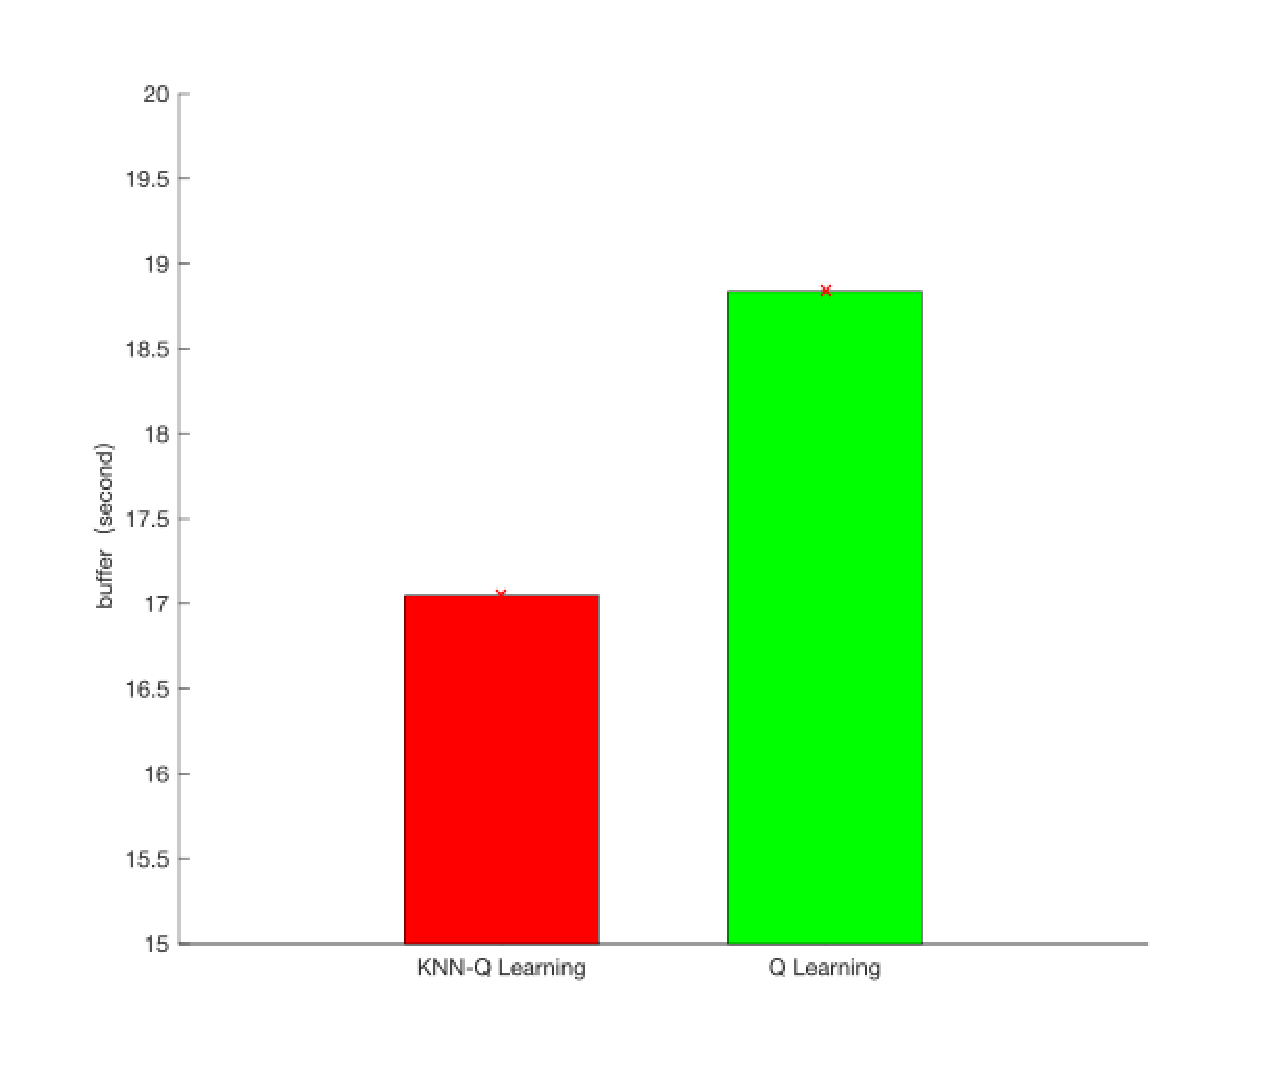
\includegraphics[width=\columnwidth]{simple_buffer_bar_graph}
\caption{简单场景buffer柱状图}
\label{simple_buffer_bar_graph}
\end{figure}
\begin{figure}[htbp]
\centering
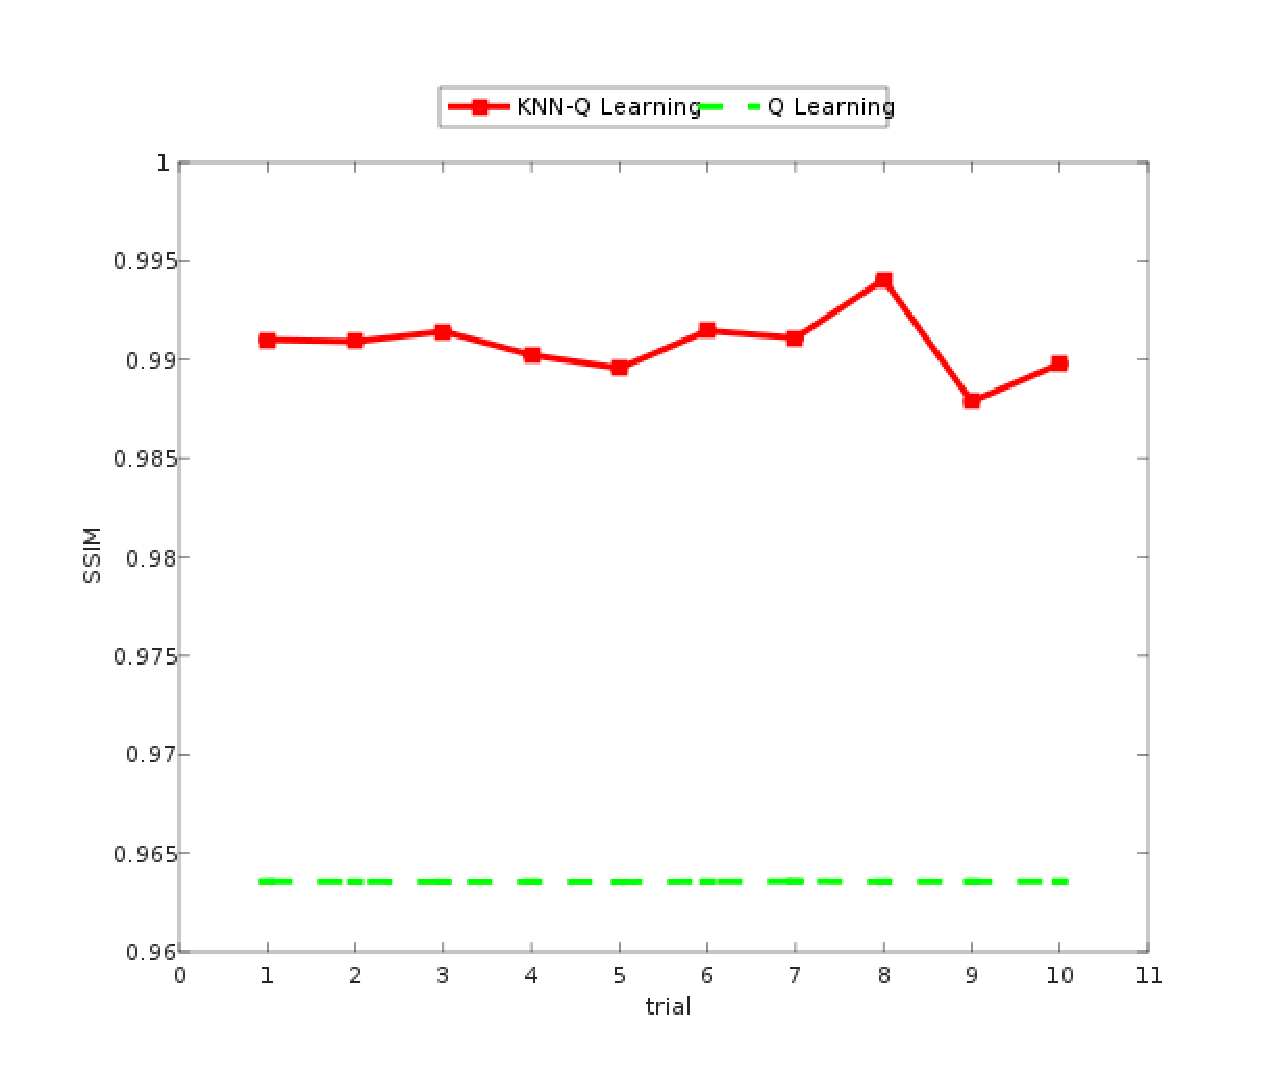
\includegraphics[width=\columnwidth]{simple_ssim_compare}
\caption{简单场景视频质量对比图}
\label{simple_ssim_compare}
\end{figure}
\begin{figure}[htbp]
\centering
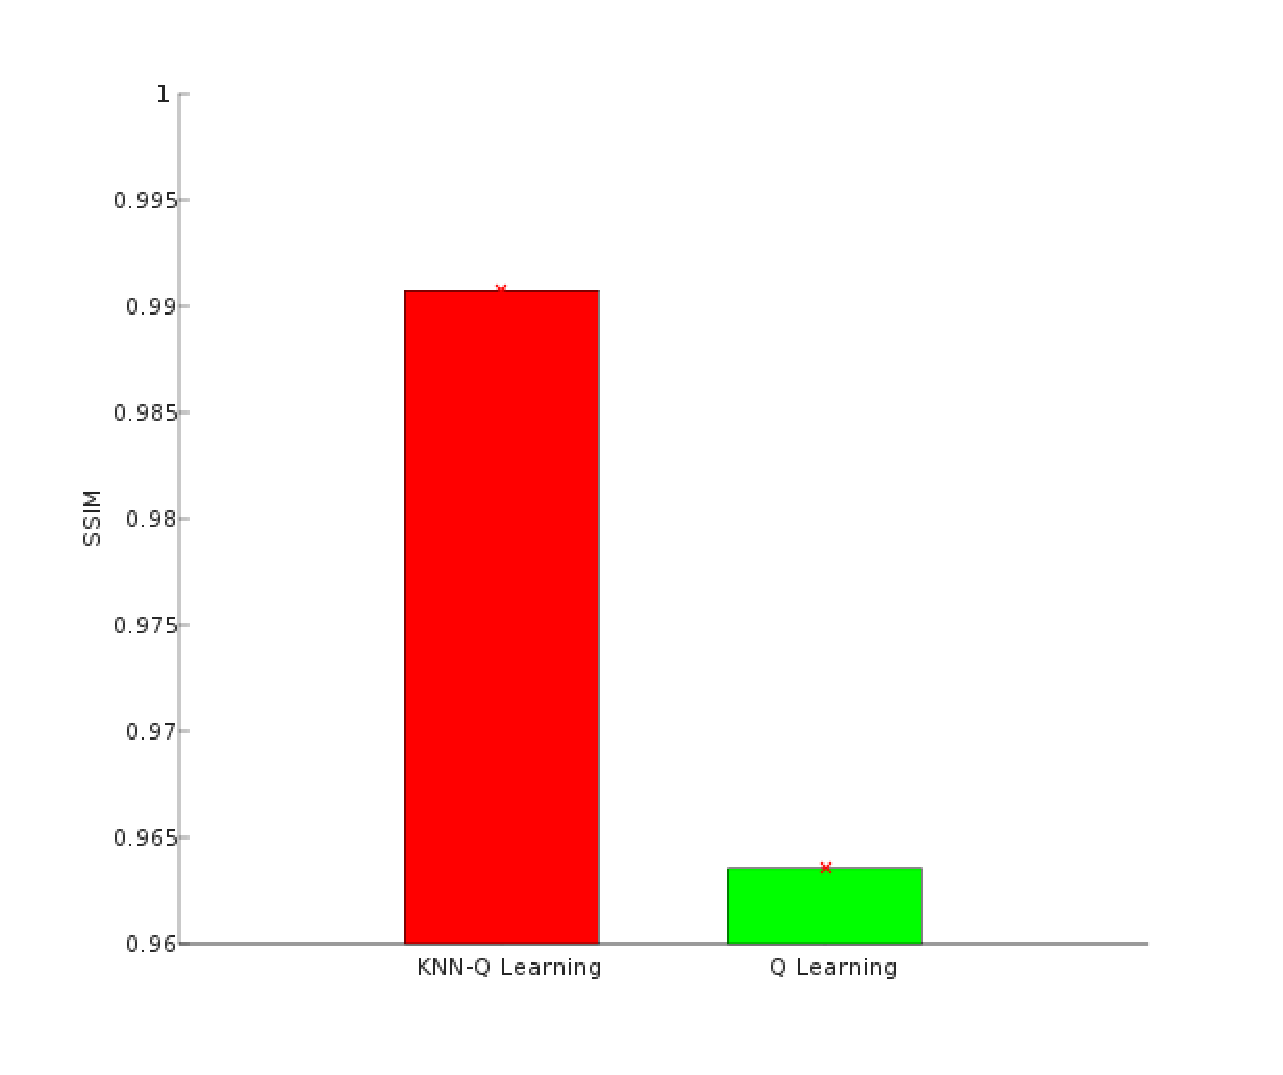
\includegraphics[width=\columnwidth]{simple_ssim_bar_graph}
\caption{简单场景平均视频质量}
\label{simple_ssim_bar_graph}
\end{figure}

\subsubsection{常规场景}
常规场景模拟显示生活中的播放视频场景,即用户带宽比较稳定,用户播放的
内容比较丰富。常规场景下利用表\ref{the SSIM value at each bit rate of 5 video materials}
中5个视频素材生成视频复杂度在波动的测试视频,网络带宽变化的范围为$\left[5000,6000\right]$,单位kb/s。

由图\ref{regular_buffer_compare}、\ref{regular_buffer_bar_graph}可知,在
常规场景下,KNN-Q学习和传统Q学习的缓存增长趋势相同,但10次平均实验没有基于Q学习
的缓存大,且两者相差近7s的缓存。

由图\ref{regular_ssim_compare}、\ref{regular_ssim_bar_graph}可知,
常规场景下,基于KNN-Q学习的码率自适应算法平均的视频质量比传统Q学习的码率自适
应算法高。
\begin{figure}[htbp]
\centering
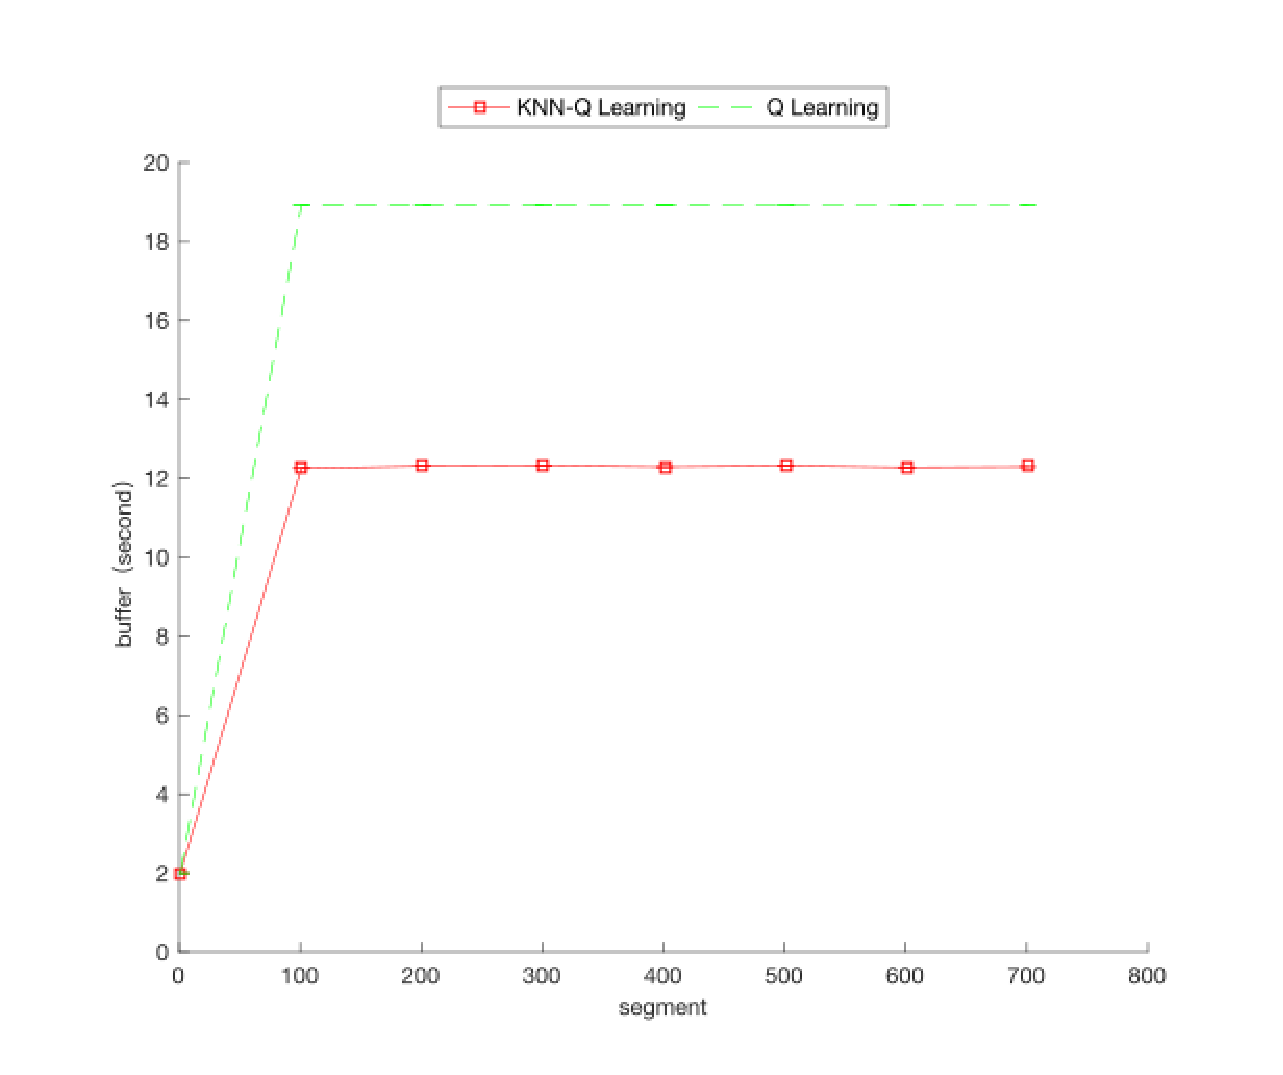
\includegraphics[width=\columnwidth]{regular_buffer_compare}
\caption{常规场景buffer趋势图}
\label{regular_buffer_compare}
\end{figure}
\begin{figure}[htbp]
\centering
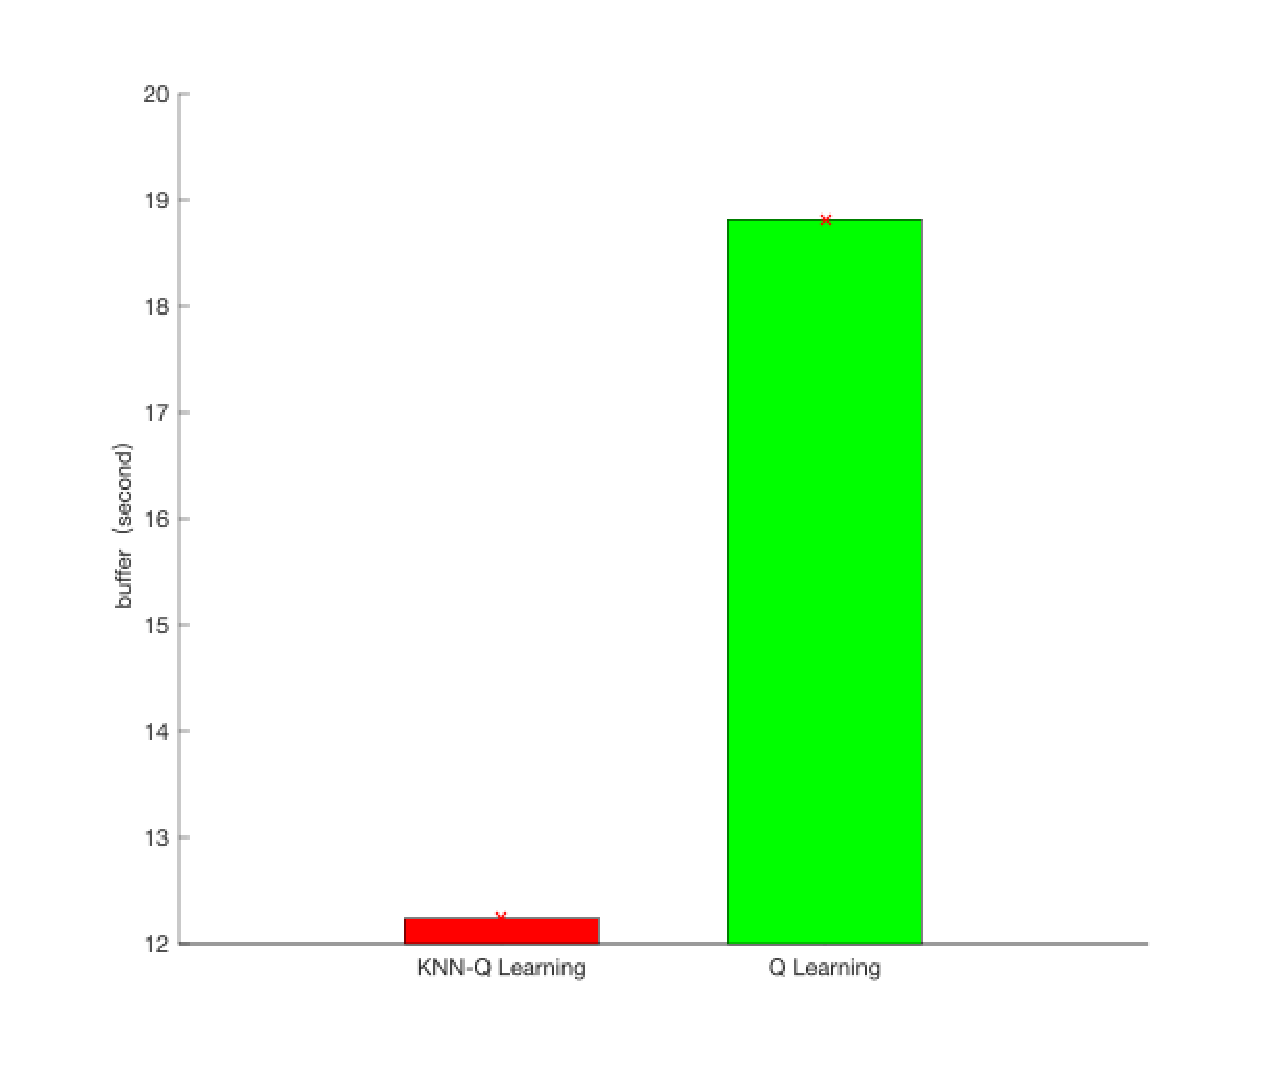
\includegraphics[width=\columnwidth]{regular_buffer_bar_graph}
\caption{常规场景buffer柱状图}
\label{regular_buffer_bar_graph}
\end{figure}
\begin{figure}[htbp]
\centering
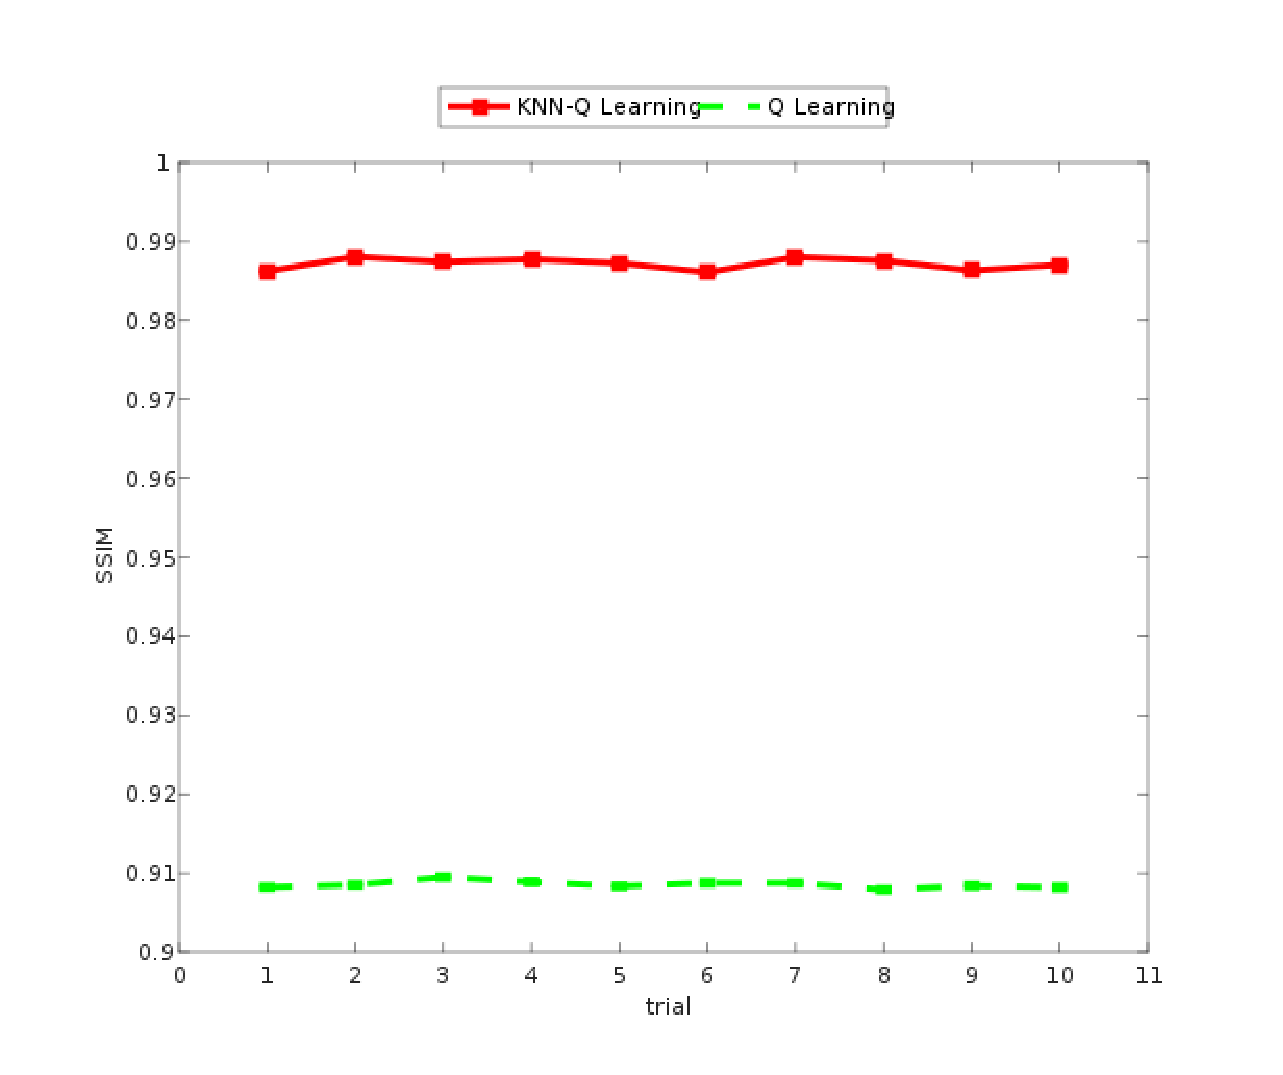
\includegraphics[width=\columnwidth]{regular_ssim_compare}
\caption{常规场景视频质量对比图}
\label{regular_ssim_compare}
\end{figure}
\begin{figure}[htbp]
\centering
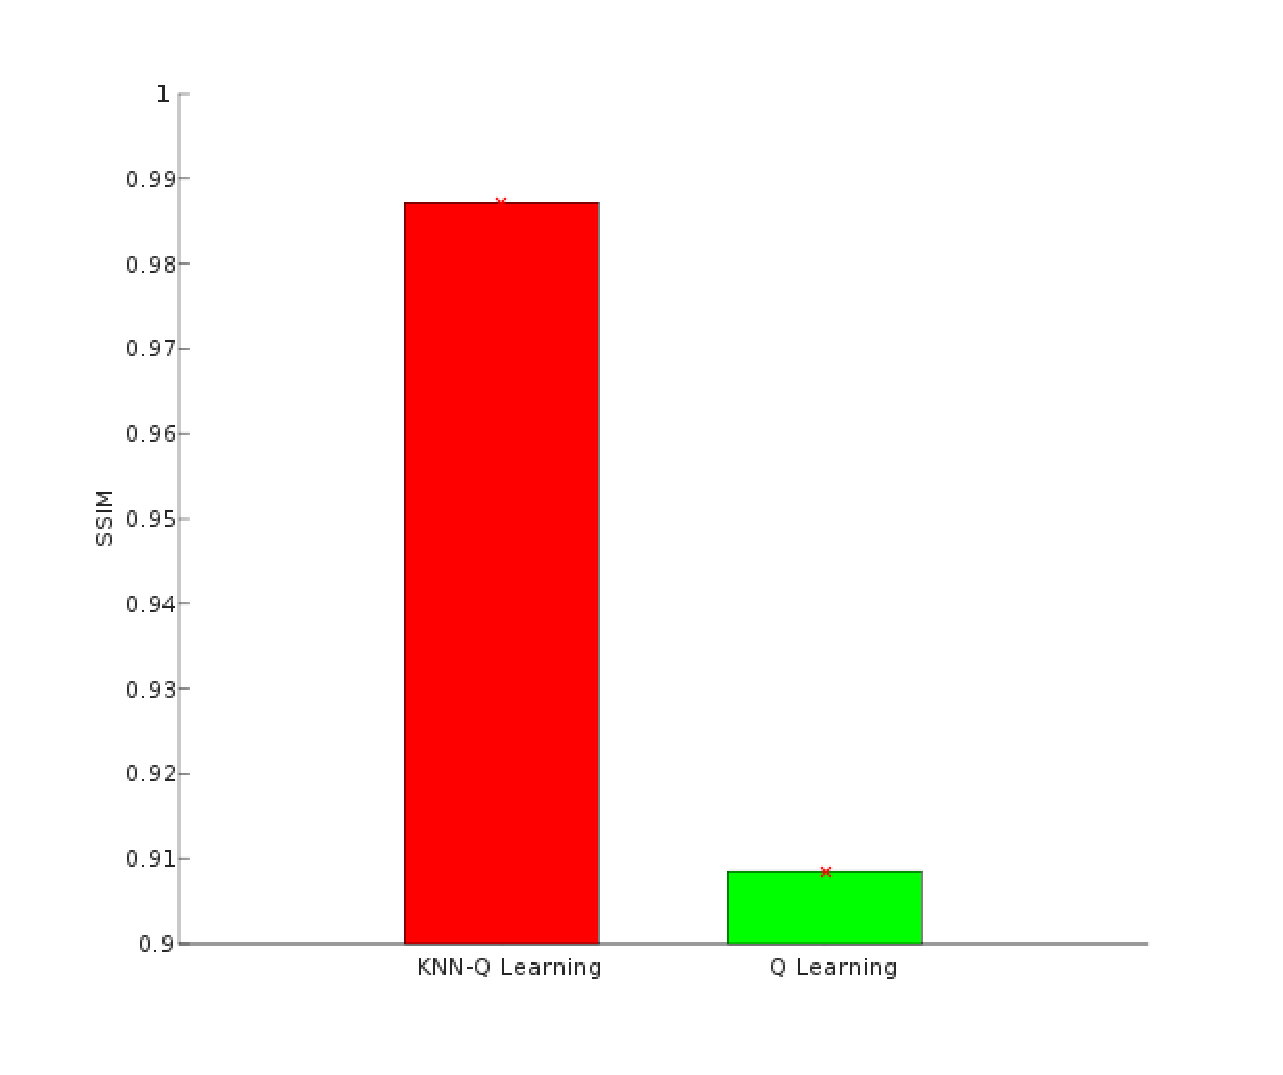
\includegraphics[width=\columnwidth]{regular_ssim_bar_graph}
\caption{常规场景平均视频质量}
\label{regular_ssim_bar_graph}
\end{figure}
\subsubsection{复杂场景}
复杂场景模拟了现实生活中网络带宽波动较大,视频内容丰富的情境。在仿真实验中,
复杂场景下模拟带宽的范围是$\left[400,12500\right]$kb/s,测试视频由表\ref{the SSIM value at each bit rate of 5 video materials}
中5个视频素材随机合成。

由图\ref{complex_buffer_compare}、\ref{complex_ssim_bar_graph}可知,在
复杂场景下,KNN-Q学习和传统Q学习的缓存增长趋势相同,但10次平均实验没有基于Q学习
的缓存大。

由图\ref{complex_ssim_compare}、\ref{complex_ssim_bar_graph}可知,
复杂场景下,基于KNN-Q学习的码率自适应算法平均的视频质量比传统Q学习的码率自适
应算法高,平均SSIM值相差近0.08。
\begin{figure}[htbp]
\centering
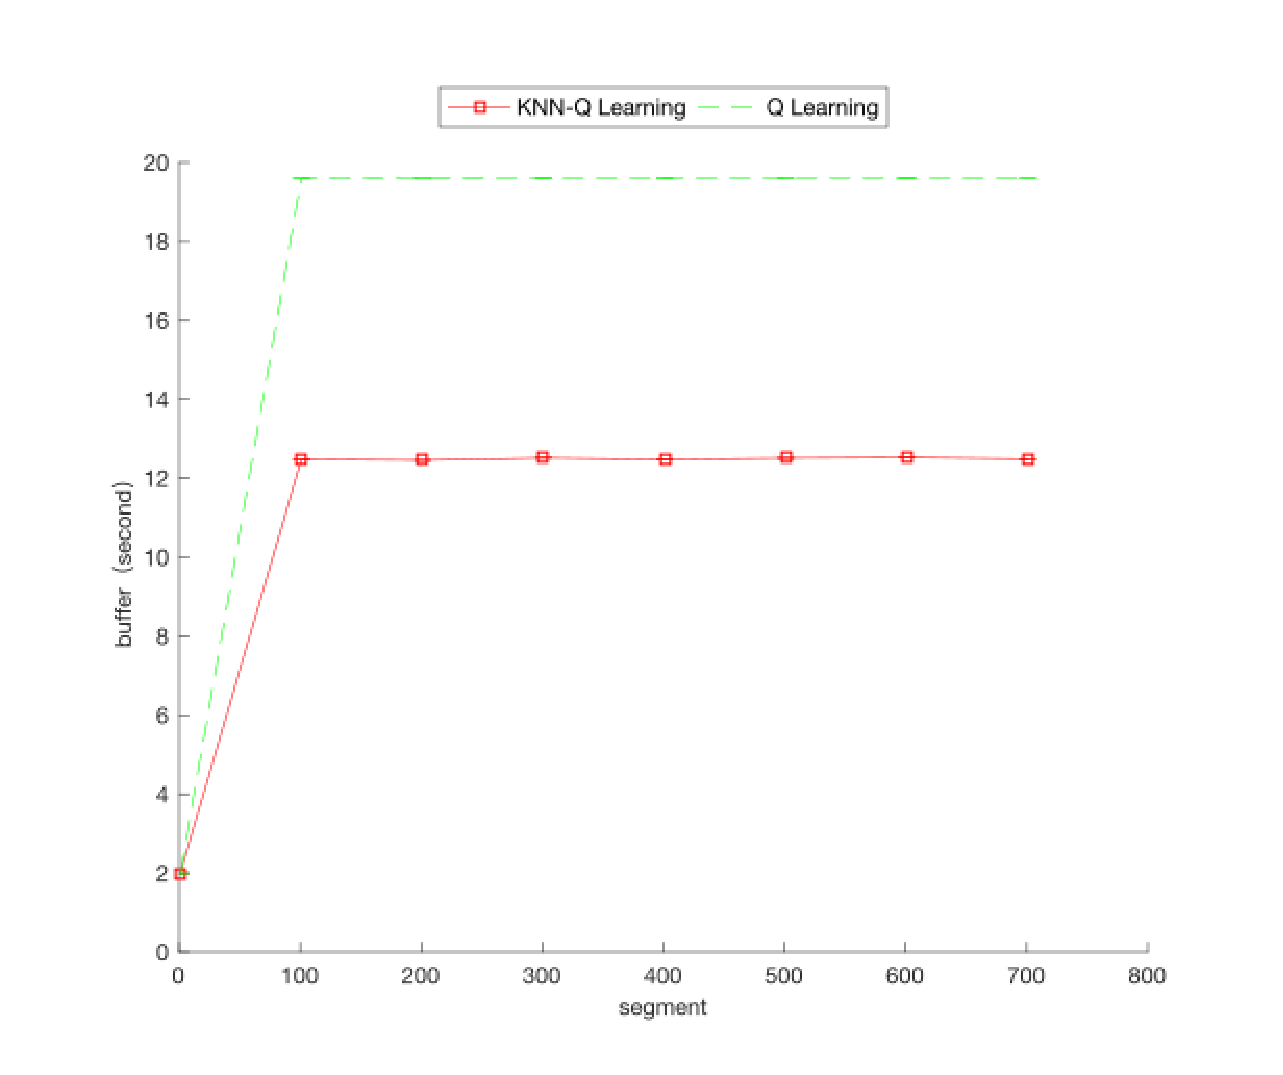
\includegraphics[width=\columnwidth]{complex_buffer_compare}
\caption{复杂场景buffer趋势图}
\label{complex_buffer_compare}
\end{figure}
\begin{figure}[htbp]
\centering
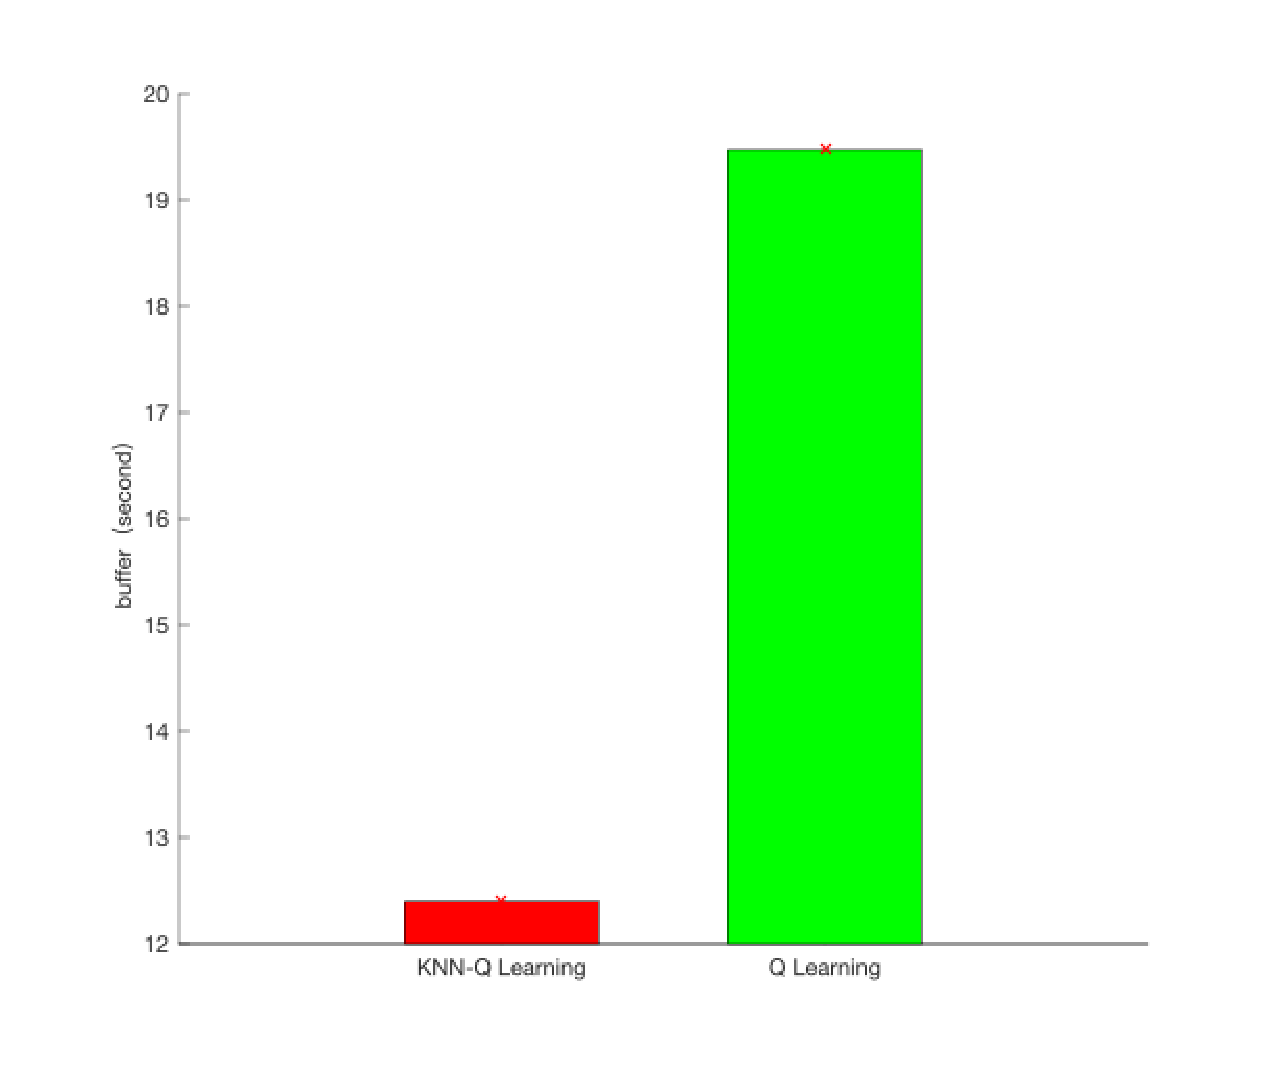
\includegraphics[width=\columnwidth]{complex_buffer_bar_graph}
\caption{复杂场景buffer柱状图}
\label{complex_buffer_bar_graph}
\end{figure}
\begin{figure}[htbp]
\centering
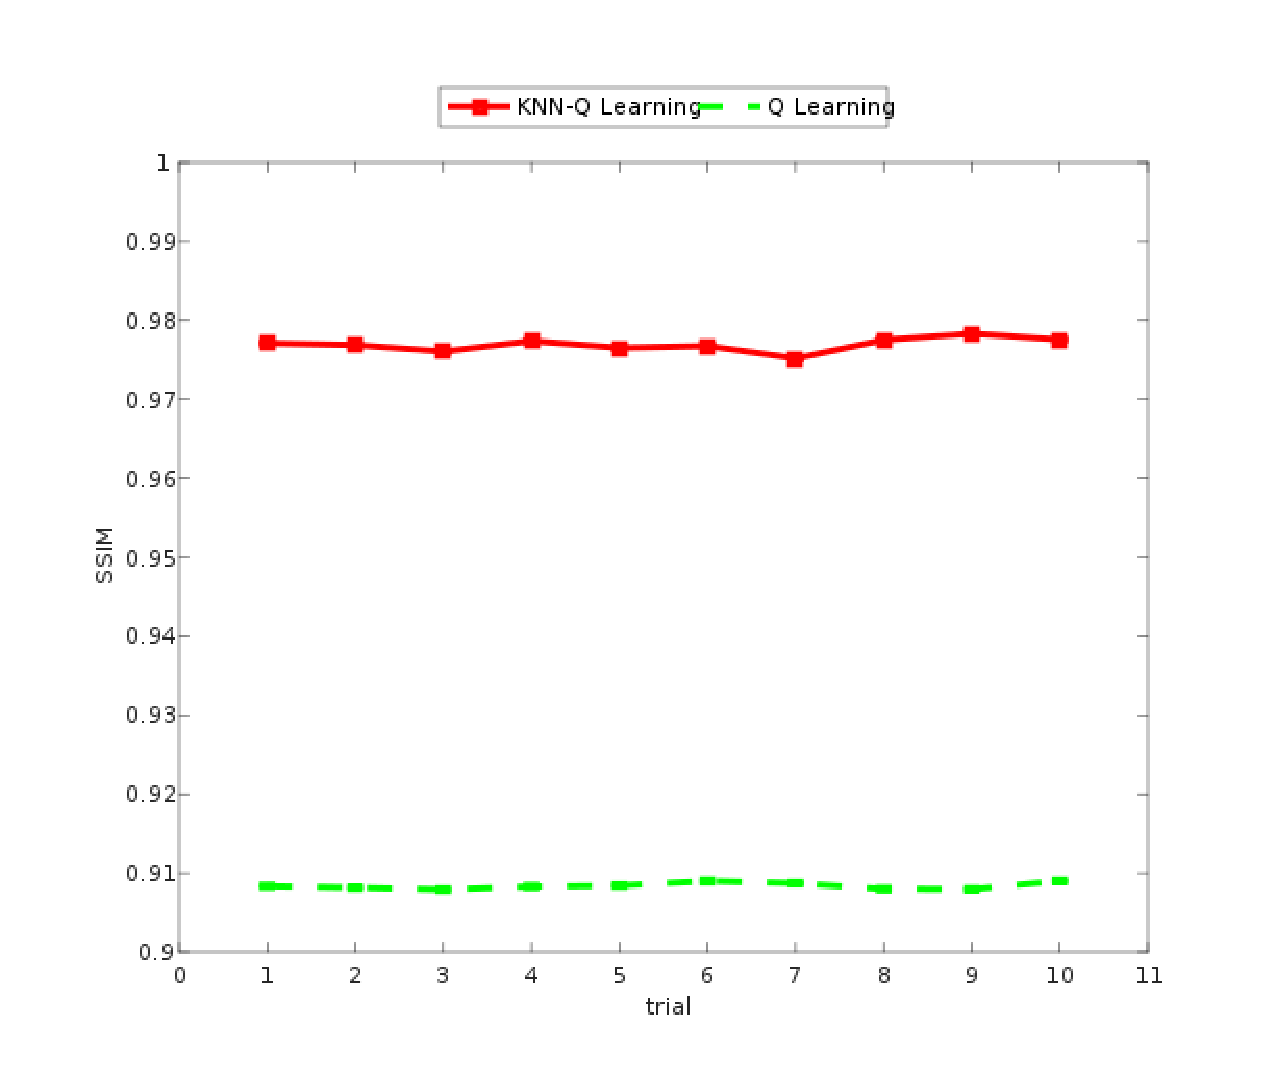
\includegraphics[width=\columnwidth]{complex_ssim_compare}
\caption{复杂场景视频质量对比图}
\label{complex_ssim_compare}
\end{figure}
\begin{figure}[htbp]
\centering
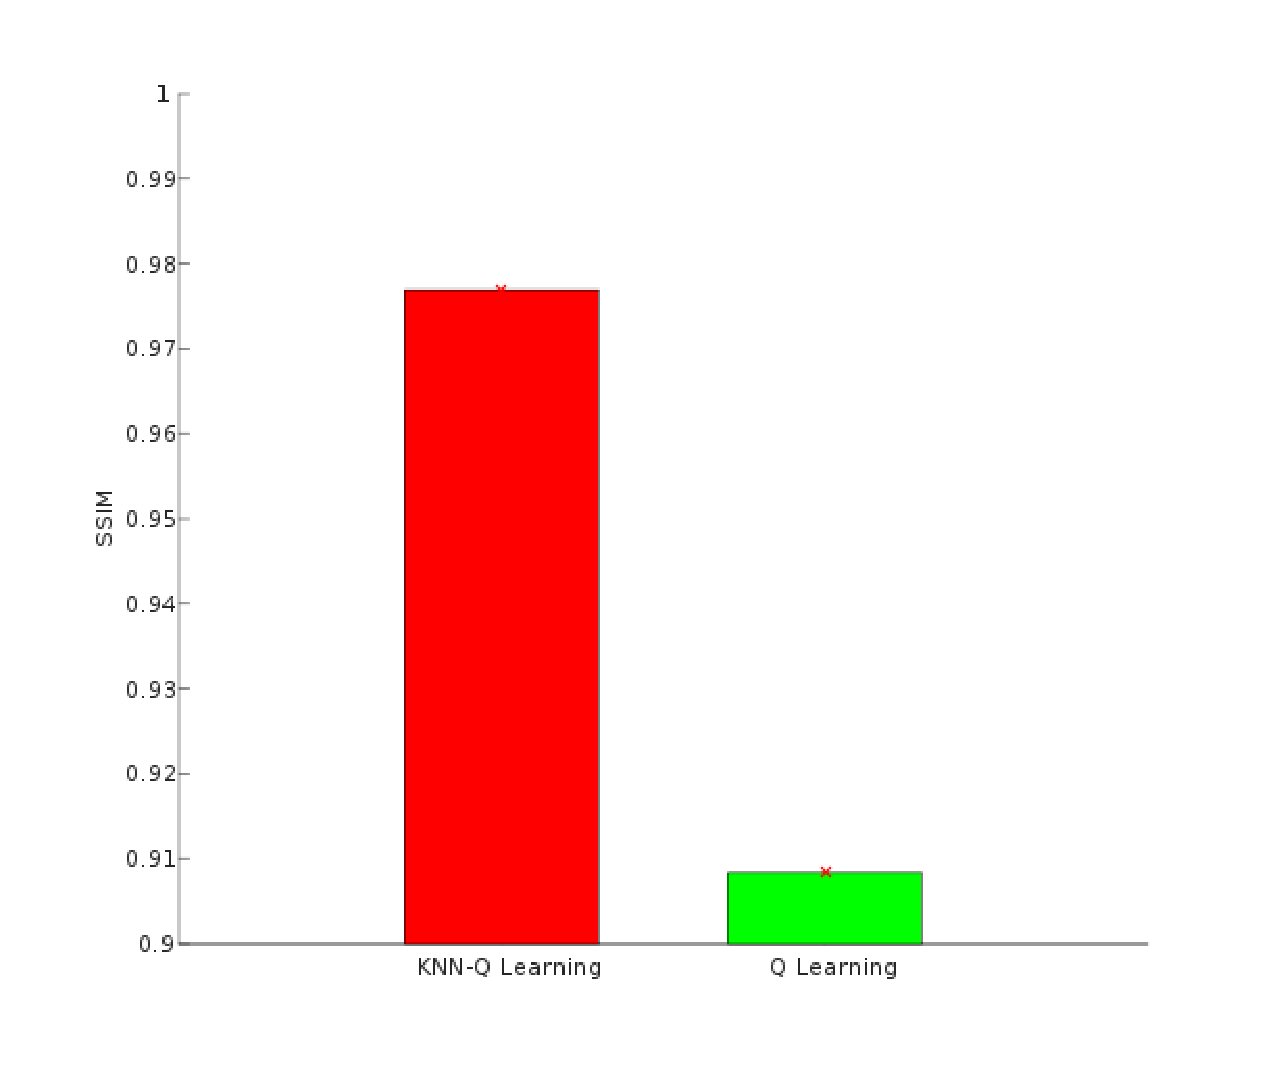
\includegraphics[width=\columnwidth]{complex_ssim_bar_graph}
\caption{复杂场景平均视频质量}
\label{complex_ssim_bar_graph}
\end{figure}

\subsubsection{K值灵敏度}
在常规场景中,设置距离公式为欧式距离,分别取K = 2,3,4,5,6
来判断KNN-Q中K值的大小对于实验效果的影响。测试视频由表\ref{the SSIM value at each bit rate of 5 video materials}
中5个视频随机合成。由图\ref{k_sensitivity_buffer}可知,K值越大,缓存也越来越大。
由图\ref{k_sensitivity_ssim}可知,K值越大,SSIM平均值越小,视频质量越差。尤其是
当K=6时,平均SSIM值迅速下降到0.91以下。
\begin{figure}[htbp]
\centering
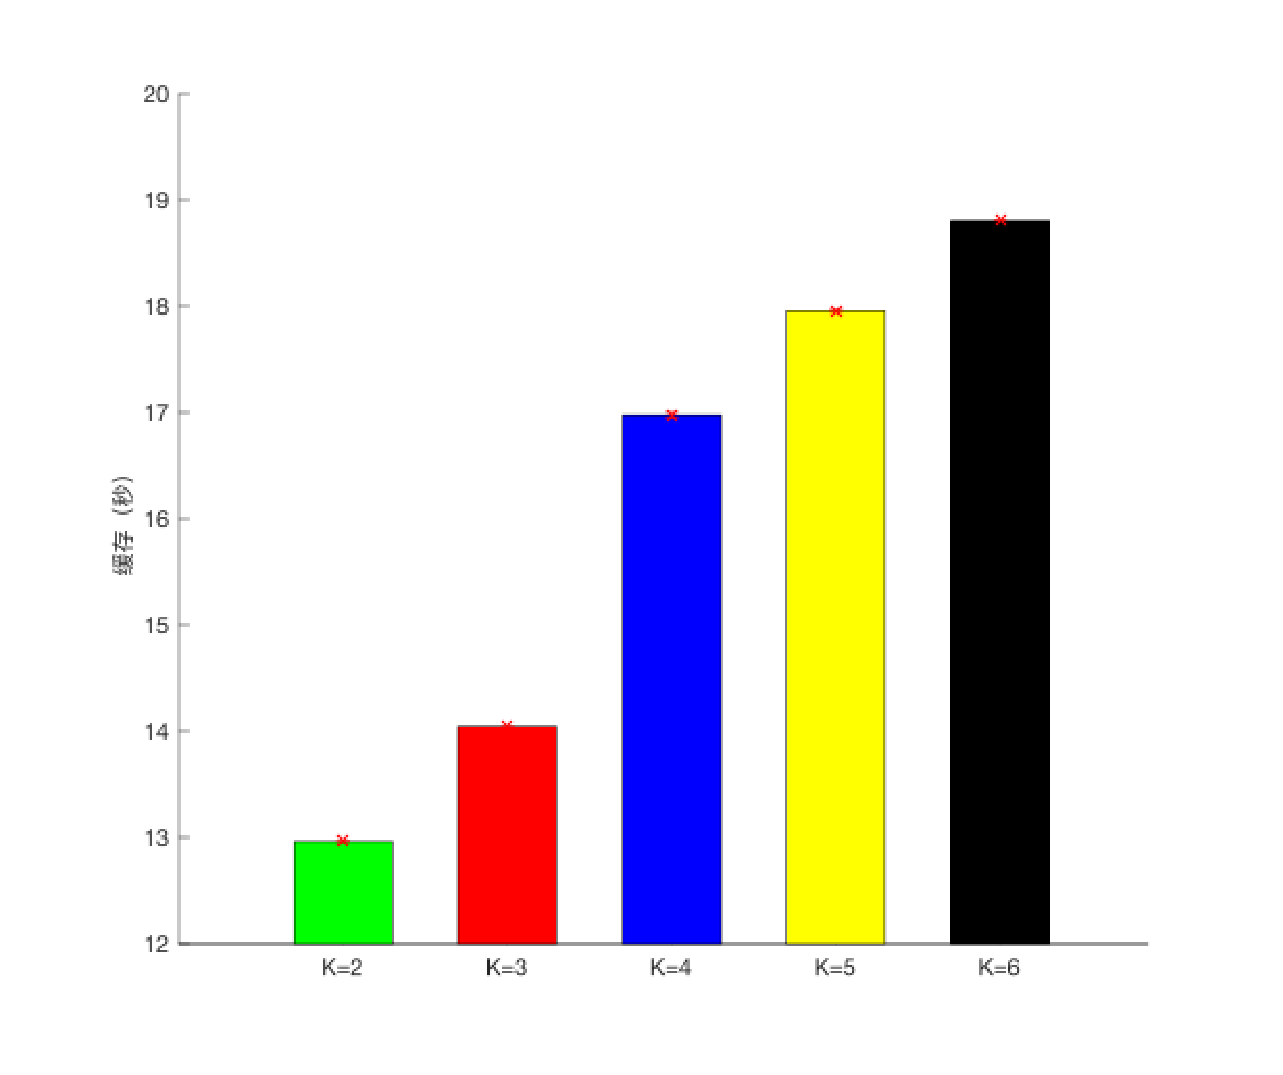
\includegraphics[width=\columnwidth]{k_sensitivity_buffer}
\caption{K值对缓存的影响}
\label{k_sensitivity_buffer}
\end{figure}
\begin{figure}[htbp]
\centering
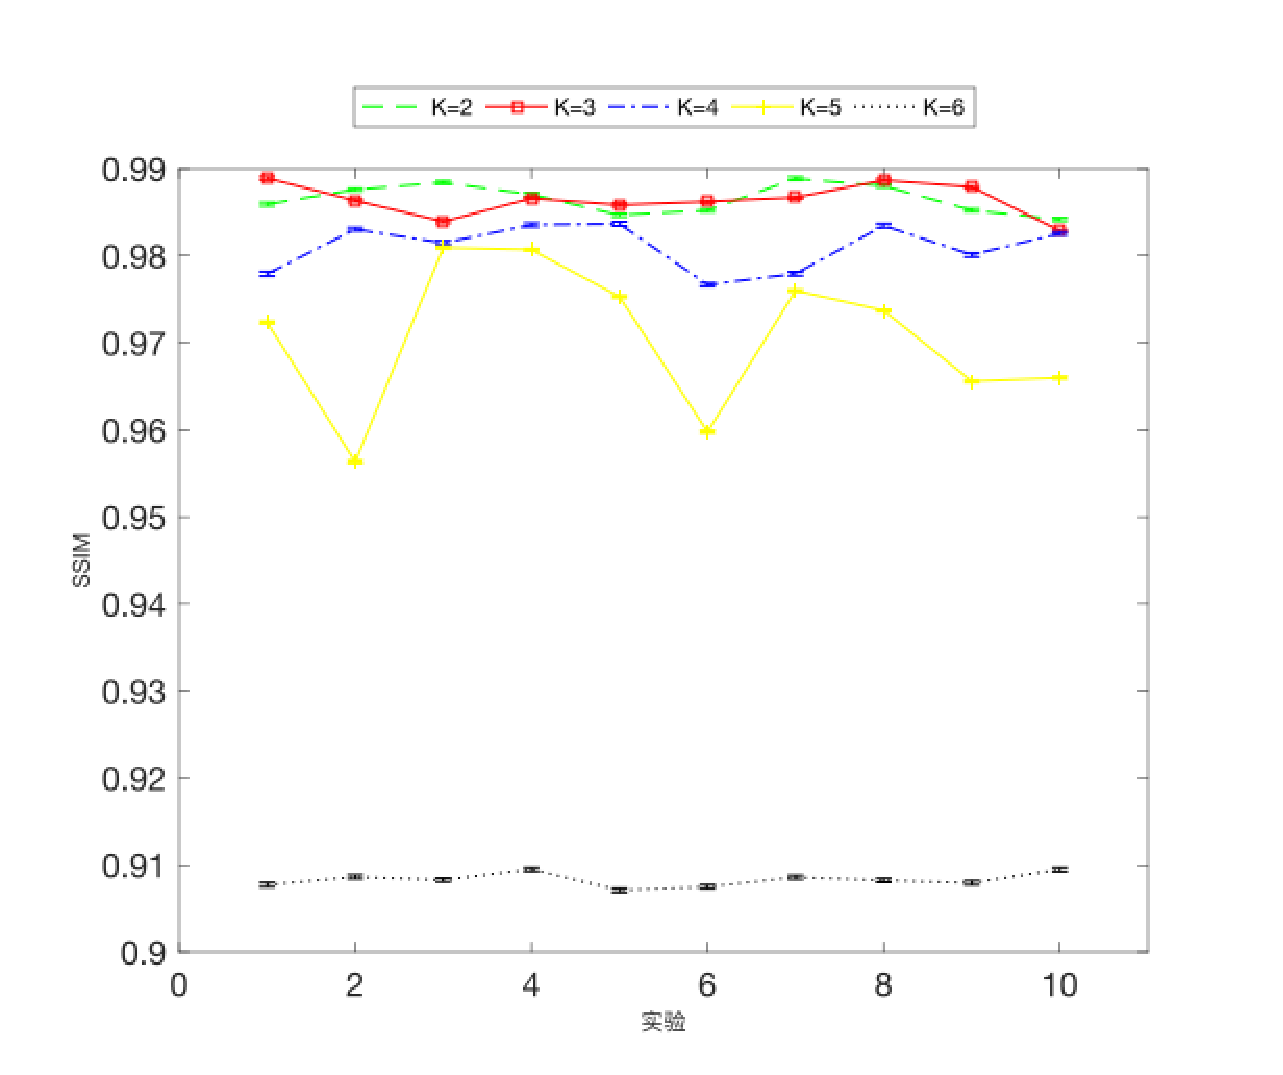
\includegraphics[width=\columnwidth]{k_sensitivity_ssim}
\caption{K值对视频质量的影响}
\label{k_sensitivity_ssim}
\end{figure}

\subsubsection{距离公式灵敏度}
在常规场景中,设置K=2。分别采用欧式距离,曼哈顿距离公式和切比雪夫
距离公式作为KNN-Q学习中的距离公式来判断KNN-Q中距离公式的选择对于实验
效果的影响。

如图\ref{distance_buffer}所示,三种距离公式对缓存几乎没有影响。
如图\ref{distance_ssim}所示,当距离公式是切比雪夫公式时,
SSIM值最低,采用欧式距离时的SSIM值最高,其次是曼哈顿距离。

\begin{figure}[htbp]
\centering
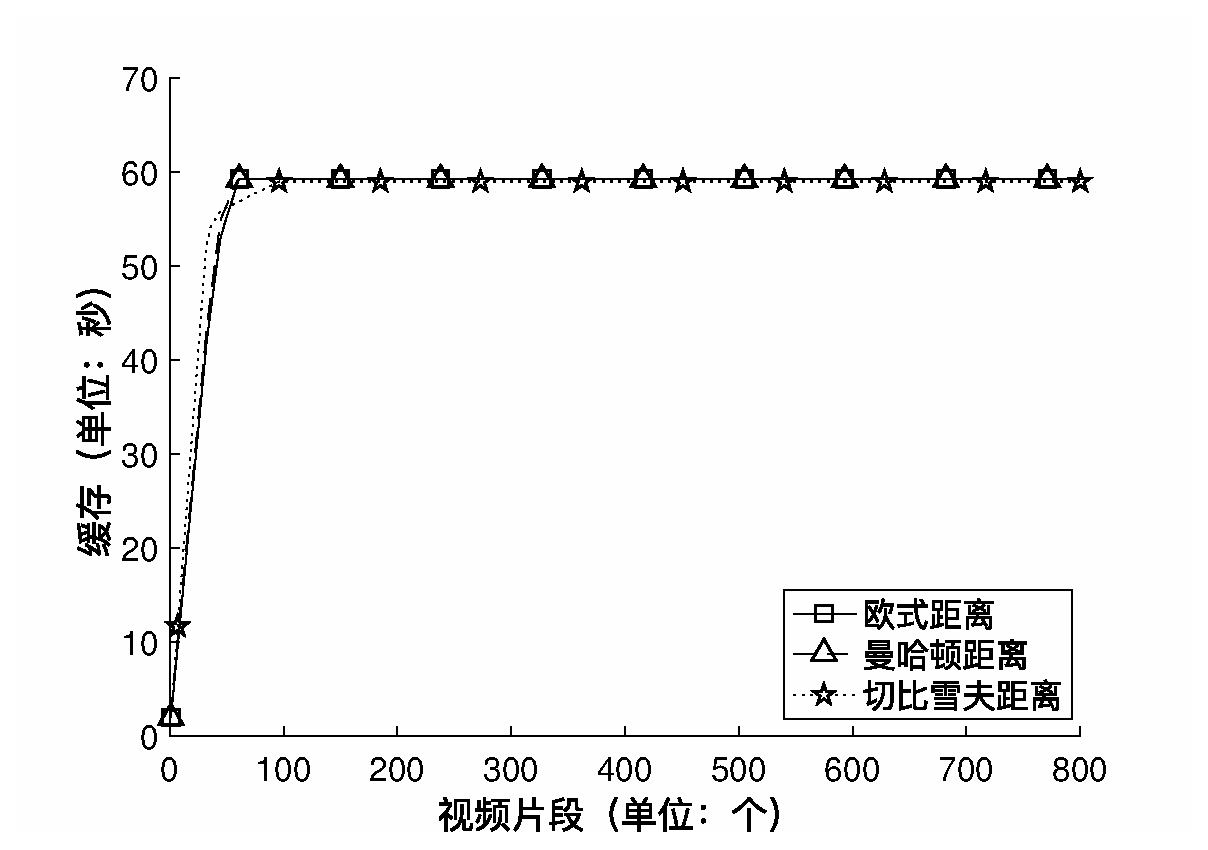
\includegraphics[width=\columnwidth]{distance_buffer}
\caption{距离公式对缓存影响}
\label{distance_buffer}
\end{figure}
\begin{figure}[htbp]
\centering
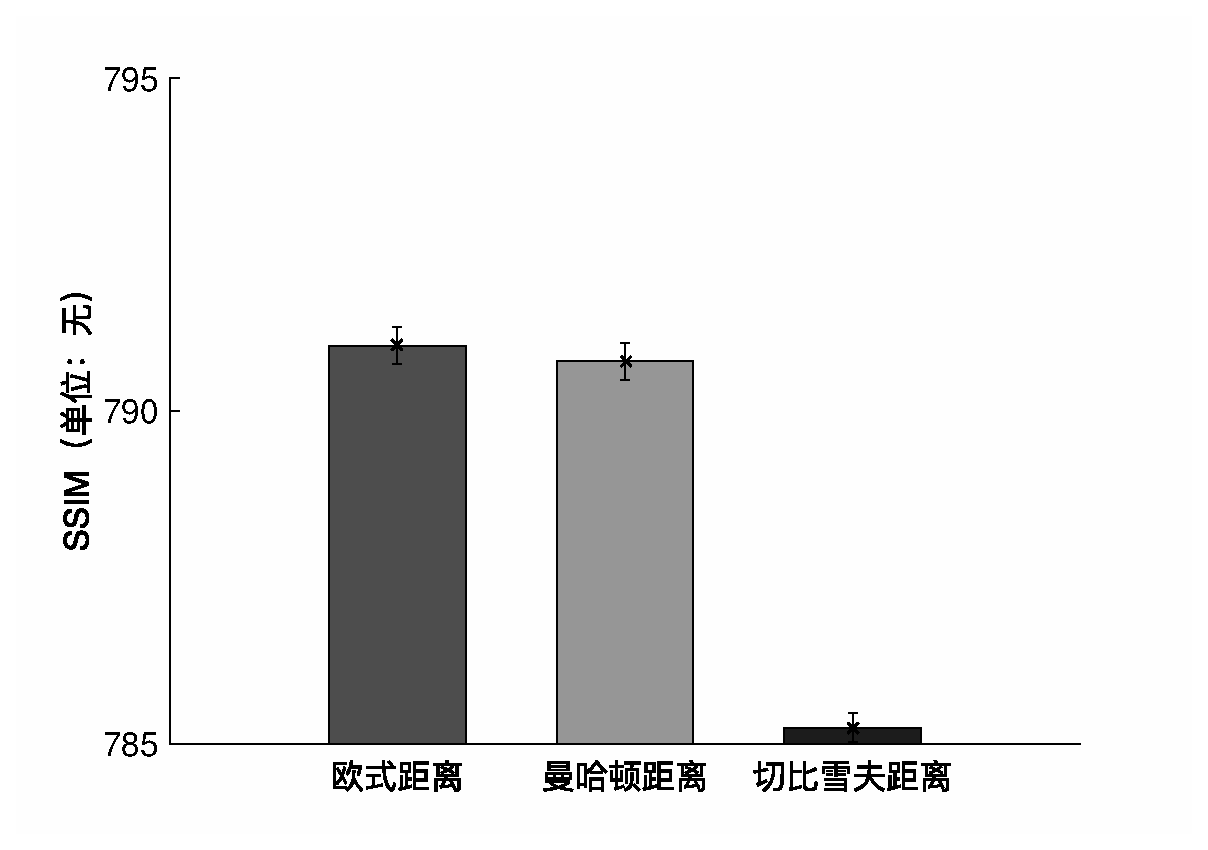
\includegraphics[width=\columnwidth]{distance_ssim}
\caption{距离公式对视频质量影响}
\label{distance_ssim}
\end{figure}
\section{结束语}
Matlab仿真实验结果显示,在简单场景、常规场景和复杂场景中,本文所提出的KNN-Q学习
码率自适应算法比传统的Q学习码率自适应算法上可以获得更高的视频质量。在训练DASH客户端
自适应策略的过程中,KNN-Q学习的收敛速度明显优于传统Q学习。在距离和公式灵敏度测试的过程中,
使用欧式距离,且K=2时,算法可以获得更高的QoE。

后续将尝试引入神经网络以替代离散的Q表来刻画连续的状态值。
\bibliographystyle{apacite}
\bibliography{mybib.bib}
\bigskip


\end{document}

